
\newif\ifcrossling\crosslingtrue
\newif\ifitmtree\itmtreetrue
\newif\iflong\longfalse
\newif\ifevaluation\evaluationfalse
\newif\ifconjugacy\conjugacyfalse
\newif\ifnonpar\nonparfalse
\newif\ifling\lingfalse
\newif\ifgibbsex\gibbsexfalse
\newif\ifhighlevel\highlevelfalse
\newif\iftmreview\tmreviewfalse
\newif\ifevocation\evocationfalse
\newif\ifsupershortmlslda\supershortmlsldatrue

\documentclass[compress]{beamer}

%\usepackage{beamerthemesplit}
\usepackage{xmpmulti}

\definecolor{green}{rgb}{0,.3,0}

\usepackage{graphicx,float,wrapfig, bbm}
\usepackage{amsfonts, bbold, comment}
\usepackage{mdwlist}
\usepackage{listings}
\usepackage{environ}
\usepackage{subfigure}
\usepackage{rotating}
\usepackage{algorithmic}
\usepackage{algorithm}
\usepackage{overpic}

\usepackage{multirow}

\usetheme[
          showdate=true,                     % show the date on the title page
          alternativetitlepage=true,         % Use the fancy title page.
          titlepagelogo=general_figures/shell,              % Logo for the fir\
st page.
          ]{UMD}


\title[]{Scalable and Efficient Probabilistic Topic Model Inference
  for Textual Data}
\author{M\r{a}ns Magnusson}
\date{Jordan Boyd-Graber}

\institute[UMD] % (optional, but mostly needed)
{Linköpings universitet}


%gets rid of bottom navigation symbols
\setbeamertemplate{navigation symbols}{}

%gets rid of footer
%will override 'frame number' instruction above
%comment out to revert to previous/default definitions
\setbeamertemplate{footline}{}


\newcommand{\explain}[2]{\underbrace{#2}_{\mbox{\footnotesize{#1}}}}
\newcommand{\dir}[1]{\mbox{Dir}(#1)}
\newcommand{\mult}[1]{\mbox{Mult}( #1)}
\newcommand{\Beta}[1]{\mbox{Beta}( #1)}
\newcommand{\G}[1]{\Gamma \left( \textstyle #1 \right)}
\newcommand{\LG}[1]{\log \Gamma \left( \textstyle #1 \right)}
\newcommand{\WN}[0]{\textsc{WordNet}}
\newcommand{\itmspace}[0]{\hspace{2cm}}
\newcommand{\abr}[1]{\textsc{#1}}
\newcommand{\lda}[0]{\abr{lda}}
\newcommand{\slda}[0]{\abr{slda}}

\newcommand{\digam}[1]{\Psi \left( \textstyle #1 \right) }
\newcommand{\ddigam}[1]{\Psi' \left( \textstyle #1 \right) }
\newcommand{\e}[2]{\mathbb{E}_{#1}\left[ #2 \right] }
\newcommand{\ind}[1]{\mathbb{I}\left[ #1 \right] }
\newcommand{\ex}[1]{\mbox{exp}\left\{ #1\right\} }
\newcommand{\D}[2]{\frac{\partial #1}{\partial #2}}
\newcommand{\elbo}{\mathcal{L}}


\newcommand{\citename}[1]{\emph{#1} }
\newcommand{\bm}[1]{\mbox{\boldmath$#1$}}
\newcommand{\Dir}{\mathrm{Dir}}
\newcommand{\Mult}{\mathrm{Mult}}
\newcommand{\g}[1]{\Gamma \left( #1 \right)}
\newcommand{\paragraph}[1]{ \vskip 1cm {\bf \large #1}}

\NewEnviron{smalign}{
\vspace{-.6cm}
\begin{small}
\begin{align}
  \BODY
\end{align}
\end{small}
\vspace{-.6cm}
}


\providecommand{\graphscale}{0.6}

\newcommand{\danquote}[1]{

\begin{flushright}
\begin{overpic}[width=5.5cm,tics=10]{general_figures/speech_bubble}
	\put(10,30) { \parbox{4cm}{#1 }}
\end{overpic}

\includegraphics[width=1.5cm]{general_figures/milkman_dan}
\end{flushright}
}


\AtBeginSection[] % "Beamer, do the following at the start of every section"
{ \begin{frame}

\frametitle{Outline} % make a frame titled "Outline"
\tableofcontents[currentsection] % show TOC and highlight current section
\end{frame} }

\lstset{language=Python,basicstyle=\tiny}

\DeclareMathSymbol{\R}{\mathbin}{AMSb}{"52}

%\setbeamertemplate{footline}{\hspace*{.5cm}\scriptsize{\insertauthor

\begin{document}

\frame{
\titlepage
\tiny
}


\section{Topic Model Introduction}



\providecommand{\graphscale}{0.6}


\newcommand{\dirfunc}[3]{ \frac{ \prod_{#1}^{#2} \g{ #3 } } { \g{ \sum_{#1}^{#2} #3 }}}
\newcommand{\dirnum}[4]{ \frac{\g{ #3 }}{#4} \prod_{#1}^{#2} }
\newcommand{\dirden}[3]{ \g{ \sum_{#1}^{#2} #3 } }



\begin{frame}

	\frametitle{Why topic models?}

	\begin{columns}

	\column{.3\linewidth}

	
\includegraphics[width=1\linewidth]{topic_models/newspapers}

	\column{.55\linewidth}

	\begin{itemize}
		\item Suppose you have a huge number of documents
		\item Want to know what's going on
		\item Can't read them all (e.g. every New York Times article from the 90's)
		\item Topic models offer a way to get a corpus-level view of major themes
		\pause
		\item Unsupervised
	\end{itemize}


	\end{columns}

\end{frame}

\frame{
\begin{center}
\frametitle{Conceptual Approach}
From an \textbf<1>{input corpus} and number of topics \textbf<1>{$K$} $\rightarrow$ \textbf<2>{words to topics} \\
\only<1>{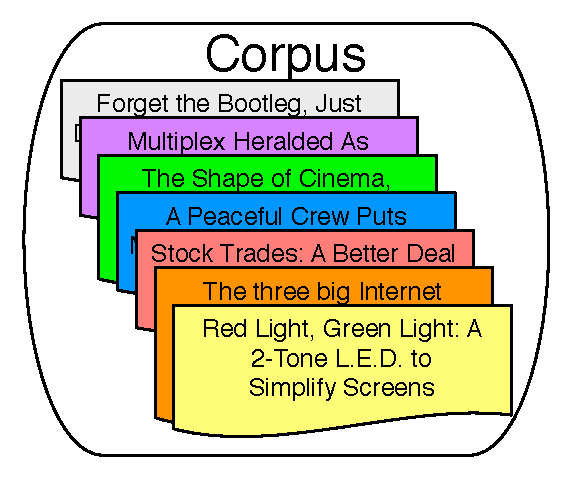
\includegraphics[width=0.6\linewidth]{reading_tea_leaves/figures/heldout_0} }
\only<2>{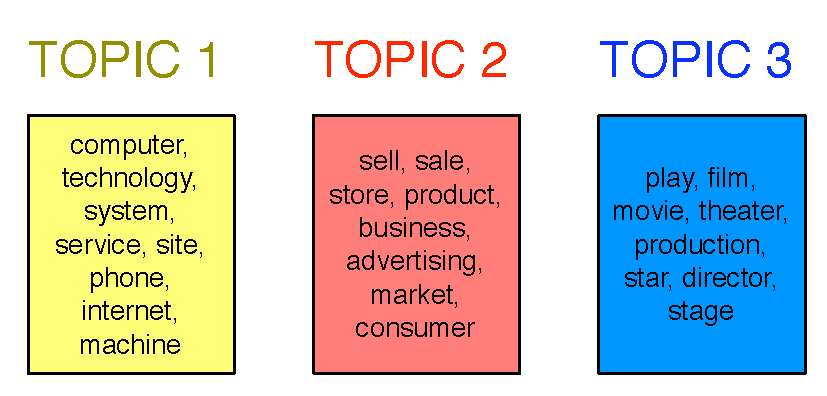
\includegraphics[width=0.9\linewidth]{reading_tea_leaves/figures/nyt_topics_wide}}
\end{center}
}

\frame{\frametitle{Conceptual Approach}

\begin{itemize}
\item For each document, what topics are expressed by that document?

\begin{center}
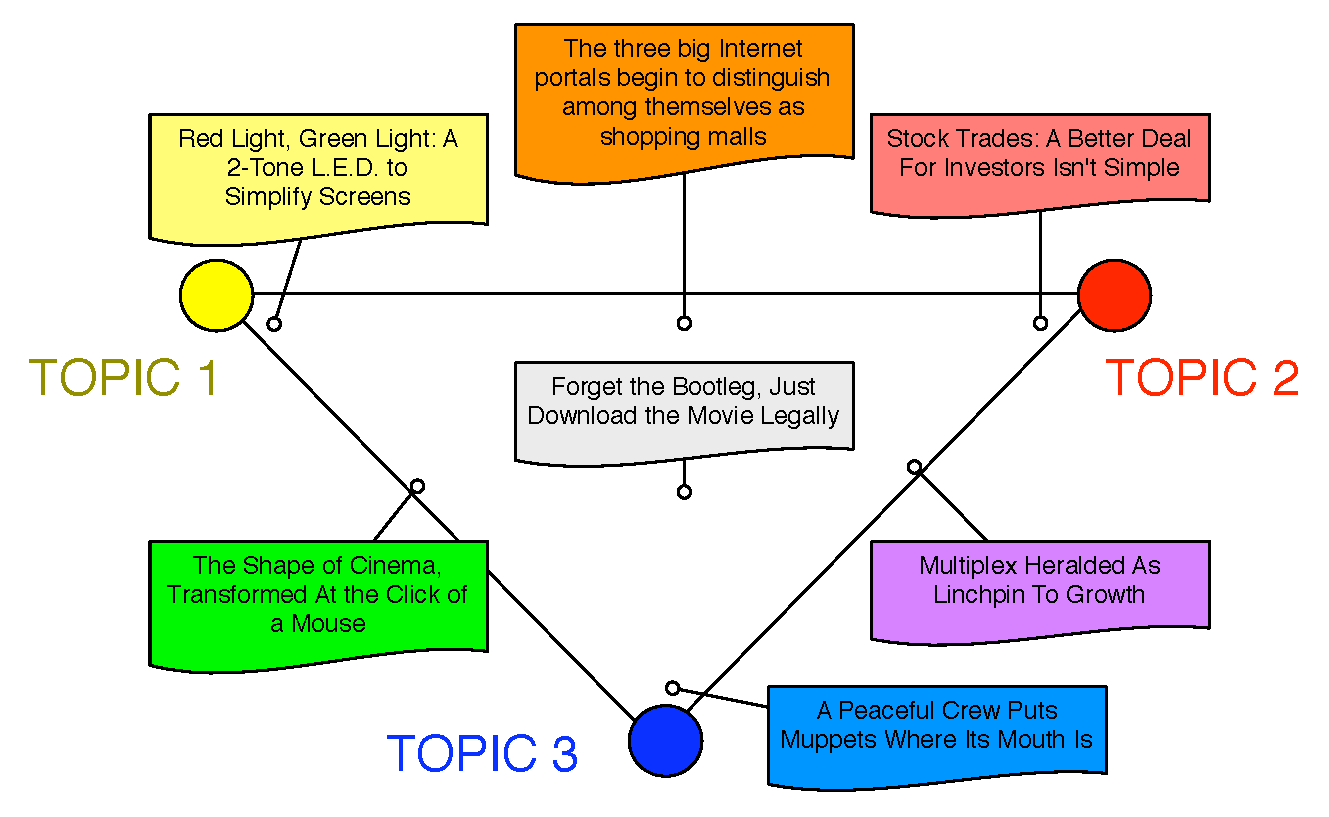
\includegraphics[width=0.9\linewidth]{topic_models/nyt_documents}
\end{center}

\end{itemize}
}


\begin{frame}

\frametitle{Topics from \emph{Science}}

\begin{center}
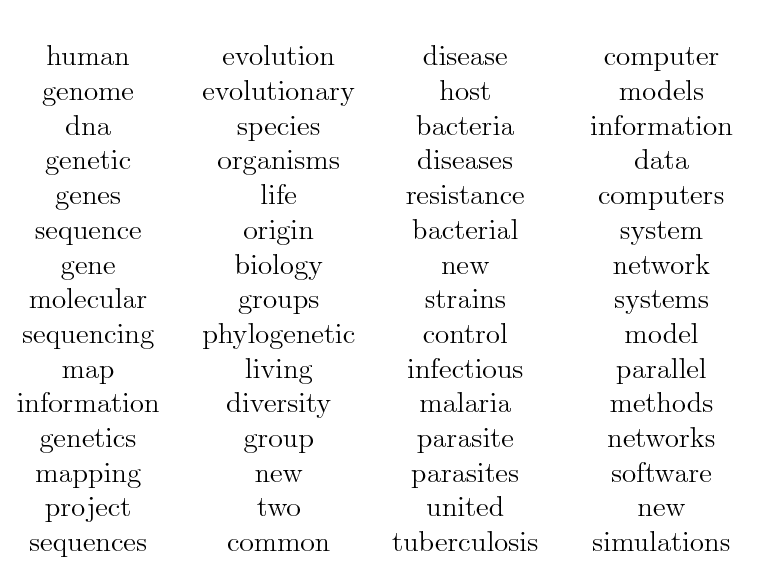
\includegraphics[width=0.8\linewidth]{topic_models/example_topics}
\end{center}

\end{frame}


\begin{frame}

\frametitle{Why should you care?}

\begin{itemize}
\item Neat way to explore / understand corpus collections
\begin{itemize}
	\item E-discovery
	\item Social media
	\item Scientific data
\end{itemize}
\item NLP Applications
\begin{itemize}
   \item POS Tagging~\cite{toutanova-08}
   \item Word Sense Disambiguation~\cite{boyd-graber-07}
   \item Word Sense Induction~\cite{brody-09}
   \item Discourse Segmentation~\cite{purver-06}
\end{itemize}
\item Psychology~\cite{griffiths-07}: word meaning, polysemy
\item Inference is (relatively) simple
\end{itemize}


\end{frame}


%\section{Definition and Derivation}



\frame
{
  \frametitle{Matrix Factorization Approach}

\begin{center}
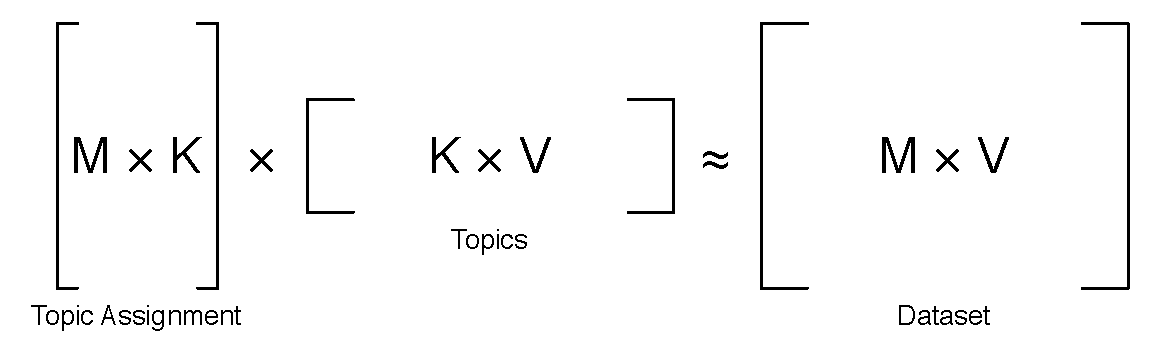
\includegraphics[width=0.9\linewidth]{topic_models/factorization.pdf}
\end{center}

\begin{columns}
\column{.5\textwidth}
\begin{block}{}
	\begin{itemize}
		\item[K] Number of topics
		\item[M] Number of documents
		\item[V] Size of vocabulary
	\end{itemize}
\end{block}
\column{.5\textwidth}
\pause
\begin{itemize}
\item If you use singular value decomposition (SVD), this technique is called latent semantic analysis.
\item Popular in information retrieval.
\end{itemize}
\end{columns}

}

\begin{frame}

\frametitle{Alternative: Generative Model}

\begin{itemize}
  \item How your data came to be
  \item Sequence of Probabilistic Steps
  \item Posterior Inference
\end{itemize}

\end{frame}

\begin{frame}
	\frametitle{Multinomial Distribution}

	\begin{itemize}
		\item Distribution over discrete outcomes
		\item Represented by non-negative vector that sums to one
		\item Picture representation
	\begin{center}
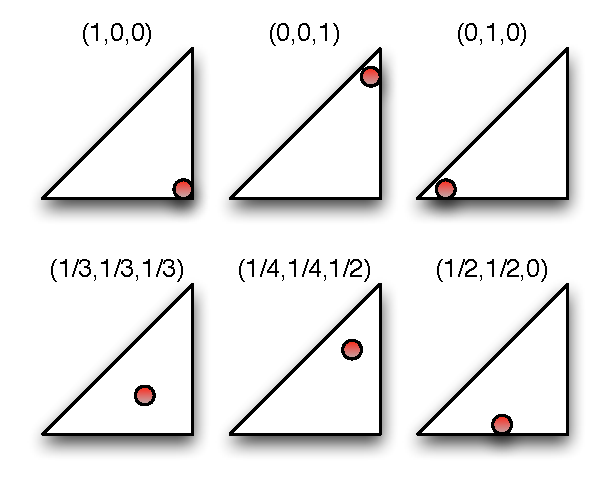
\includegraphics[width=0.4\linewidth]{topic_models/multinomial}
	\end{center}
		\pause
		\item Come from a Dirichlet distribution

	\end{itemize}

        \pause

        \vspace{-5cm}

        \begin{block}{Look familiar?}
          \centering
          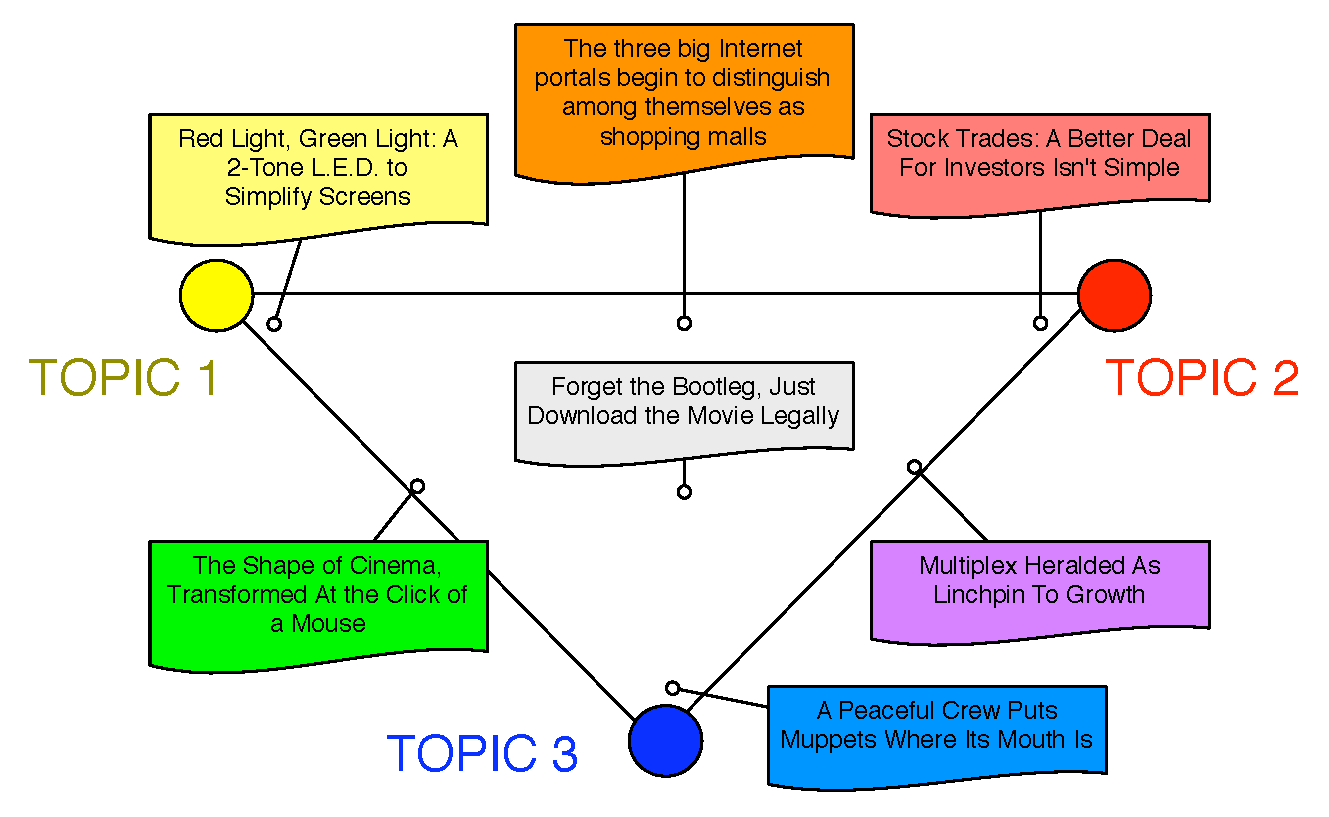
\includegraphics[width=0.7\linewidth]{topic_models/nyt_documents}
        \end{block}

\end{frame}

\begin{frame}

\frametitle{Dirichlet Distribution}

\begin{center}
\begin{equation}
  p(\theta | \vec{\alpha}) = \frac{ \Gamma \left( \sum_k \alpha_k \right)}{\prod_k \Gamma(\alpha_k)} \prod_k \theta_k^{\alpha_k = 1}
\end{equation}
\bigskip

\only<2>{

\includegraphics[width=0.6\linewidth]{topic_models/dirichlet_1} \\
\begin{tabular}{ccc}
$\vec \alpha = \left(\frac{1}{3}, \frac{1}{3}, \frac{1}{3} \right)$ &
$\vec \alpha = \left(2, 2, 2 \right)$ & 
$\vec \alpha = \left(10, 10, 10 \right)$  \\
\end{tabular} }

\only<3>{

\includegraphics[width=0.6\linewidth]{topic_models/dirichlet_2} \\
\begin{tabular}{ccc}
$\vec \alpha = \left(2, 10, 2 \right)$ & 
$\vec \alpha = \left(2, 2, 10 \right)$ & 
$\vec \alpha = \left(\frac{4}{5}, \frac{4}{5}, \frac{4}{5} \right)$  \\
\end{tabular} }

\end{center}

\end{frame}

\begin{frame}
\frametitle{Dirichlet Distribution}
\begin{center}
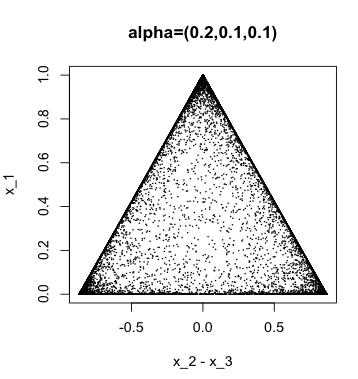
\includegraphics[width=0.5\linewidth]{topic_models/sparsity}
\end{center}
\end{frame}

\fi
\ifconjugacy

\begin{frame}
\frametitle{Dirichlet Distribution}
\begin{itemize}
  \item If ${\bm \phi} \sim \Dir(\alpha)$, ${\bm w} \sim \Mult(\phi)$, and $n_k = |\{ w_i : w_i = k\}|$ then
  \begin{align}
  	p(\phi | \alpha, {\bm w}) & \propto p({\bm w} | \phi) p(\phi | \alpha) \\
	                       & \propto  \prod_{k} \phi^{n_k} \pause  \prod_k { \phi^{\alpha_k - 1}} \\
	                       & \propto \prod_k \phi^{\alpha_k + n_k - 1}
  \end{align}
  \item Conjugacy: this {\bf posterior} has the same form as the {\bf prior}
\end{itemize}
\end{frame}

\fi

\ifhighlevel

\else

\frame
{
  \frametitle{Generative Model Approach}

\begin{center}
\only<1>{ 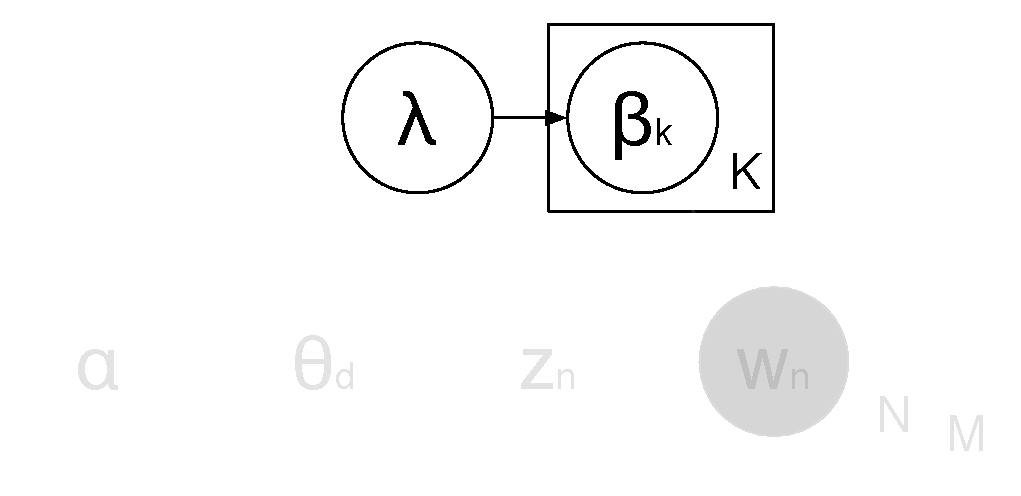
\includegraphics[scale=0.4]{topic_models/lda1.pdf} }
\only<2>{ 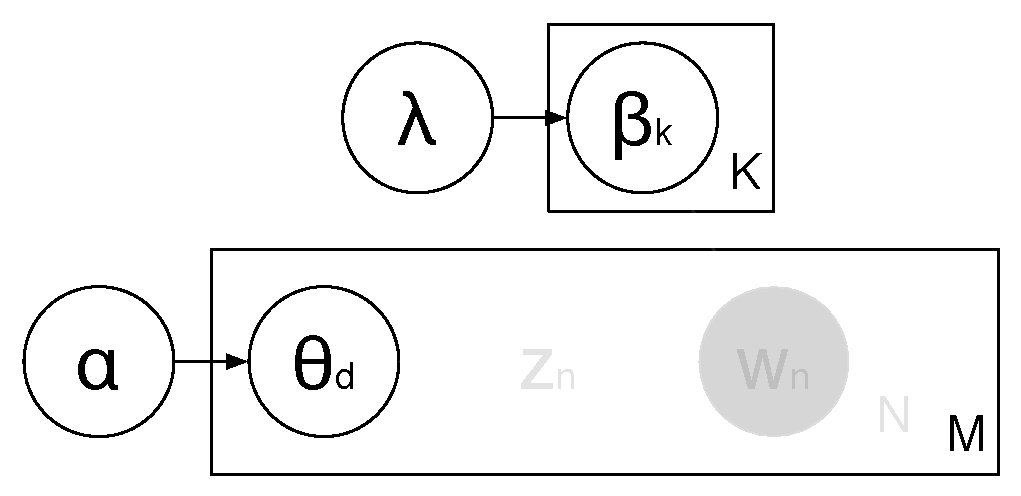
\includegraphics[scale=0.4]{topic_models/lda2.pdf} }
\only<3>{ 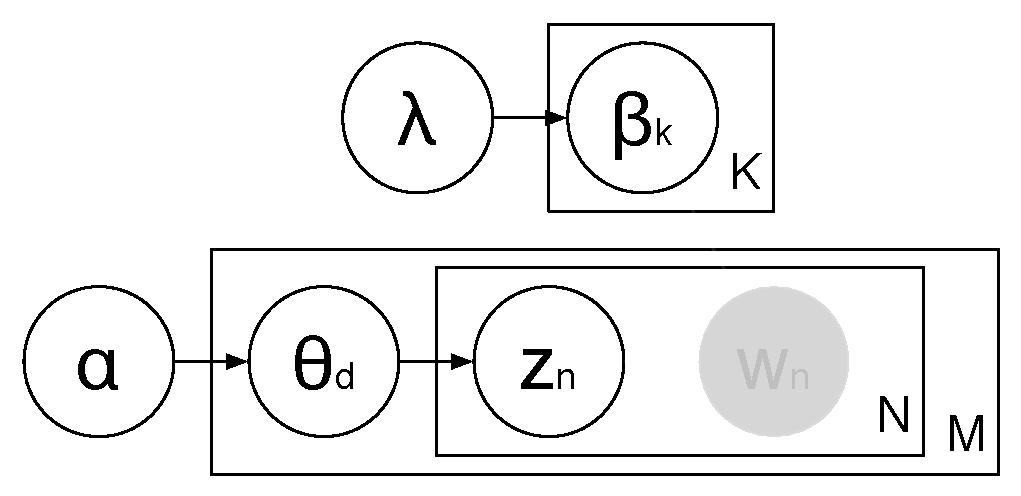
\includegraphics[scale=0.4]{topic_models/lda3.pdf} }
\only<4->{ 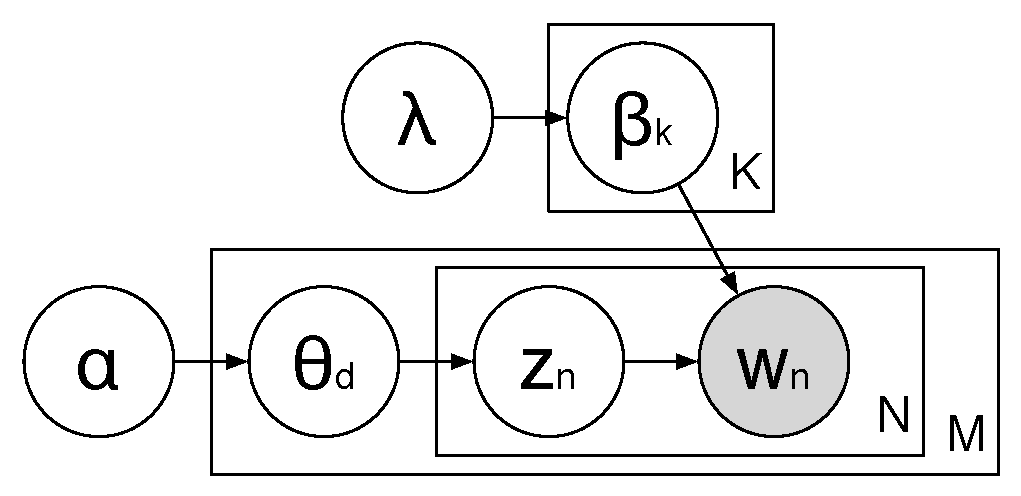
\includegraphics[scale=0.4]{topic_models/lda4.pdf} }
\end{center}

\begin{itemize}
\item<1-> For each topic $k \in \{1, \dots, K\}$, draw a multinomial distribution $\beta_k$ from a Dirichlet distribution with parameter $\lambda$
\item<2-> For each document $d \in \{1, \dots, M\}$, draw a multinomial distribution $\theta_d$ from a Dirichlet distribution with parameter $\alpha$
\item<3-> For each word position $n \in \{1, \dots, N\}$, select a hidden topic $z_n$ from the multinomial distribution parameterized by $\theta$.
\item<4-> Choose the observed word $w_n$ from the distribution $\beta_{z_n}$.
\end{itemize}

\only<5->{We use statistical inference to uncover the most likely unobserved variables given observed data.}
}

\fi

\begin{frame}
\frametitle{Topic Models: What's Important}
\begin{itemize}
\item Topic models \only<2>{(latent variables)}
\begin{itemize}
\ifhighlevel
	\item Topics to words
	\item Documents to topics
\else
	\item Topics to words---multinomial distribution
	\item Documents to topics---multinomial distribution
\fi
\end{itemize}
\item Focus in this talk: statistical methods
  \begin{itemize}
    \item Model: story of how your data came to be
    \item Latent variables: missing pieces of your story
    \item Statistical inference: filling in those missing pieces
  \end{itemize}
\item We use latent Dirichlet allocation (LDA)~\cite{blei-03}, a fully Bayesian
  version of pLSI~\cite{hofmann-99}, probabilistic version of
  LSA~\cite{landauer-97}
\end{itemize}

\end{frame}

\ifevaluation


\frame{
\frametitle{Evaluation}
\begin{center}
%\only<1>{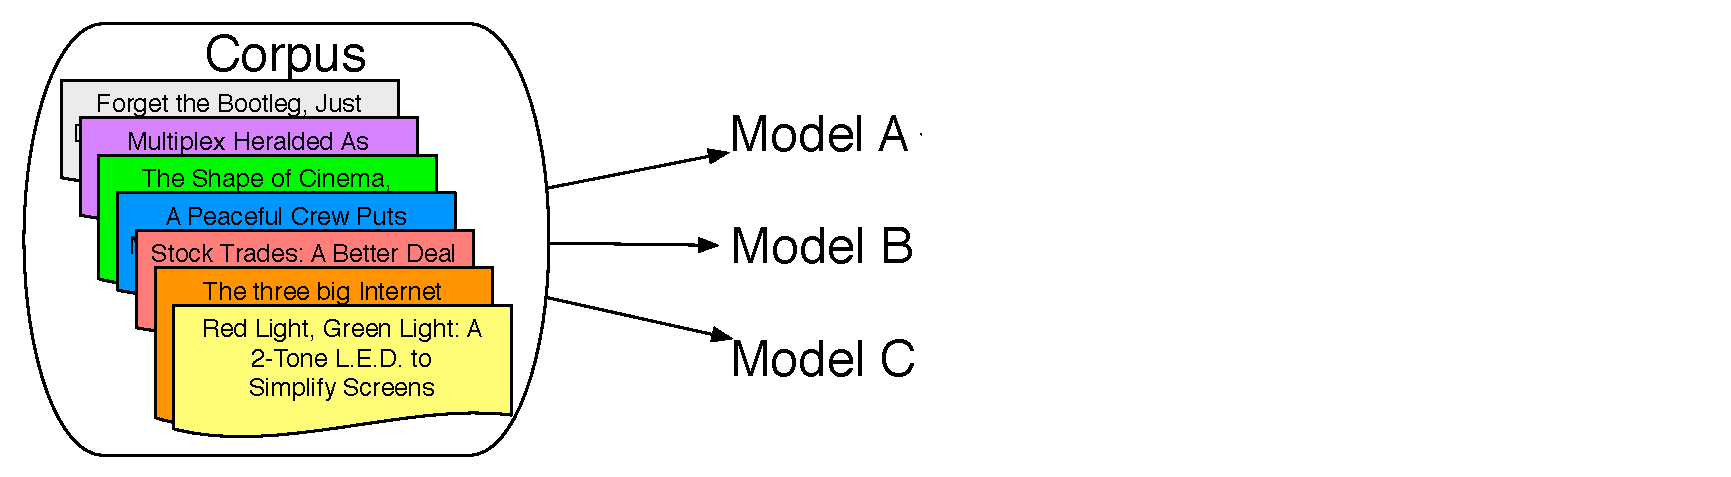
\includegraphics[width=0.9\linewidth]{reading_tea_leaves/figures/heldout_1} }
\only<1>{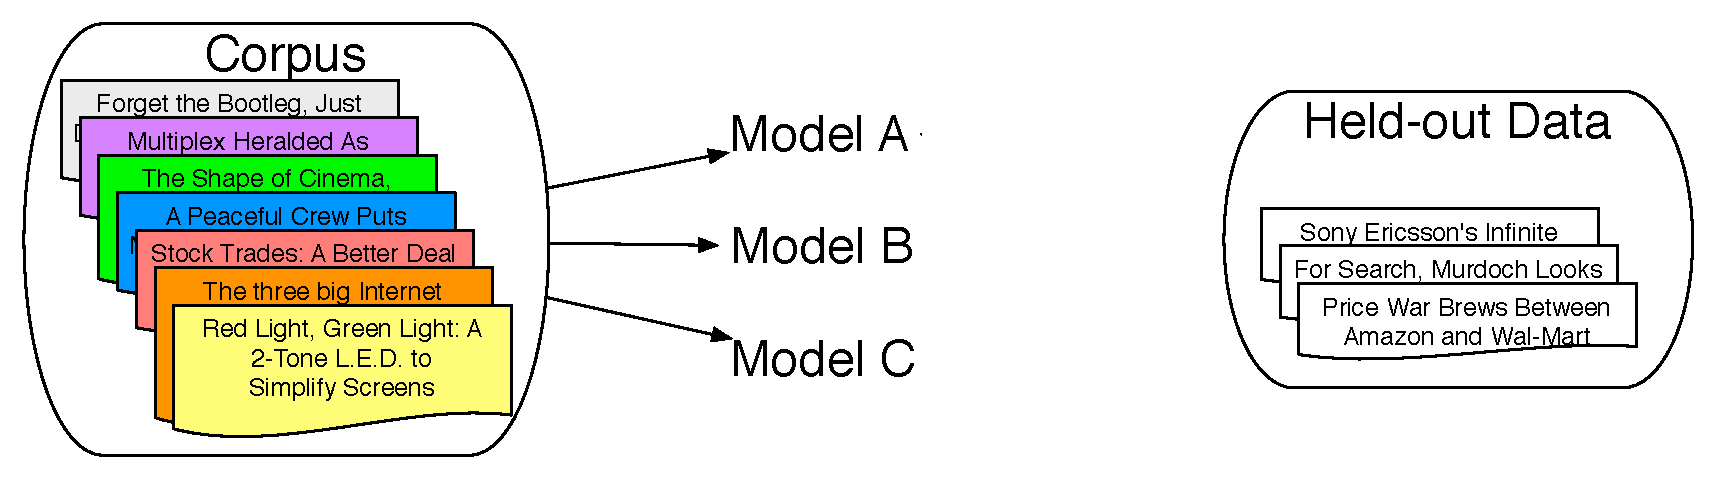
\includegraphics[width=\linewidth]{reading_tea_leaves/figures/heldout_2} }
%\only<3>{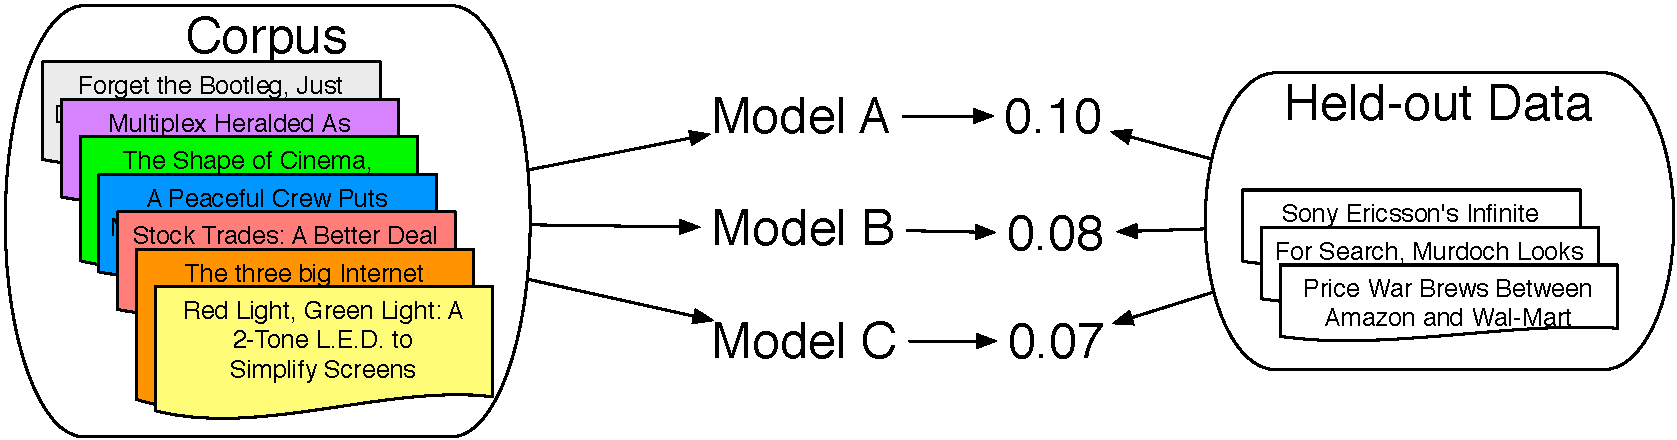
\includegraphics[width=\linewidth]{reading_tea_leaves/figures/heldout_3} }
\only<2>{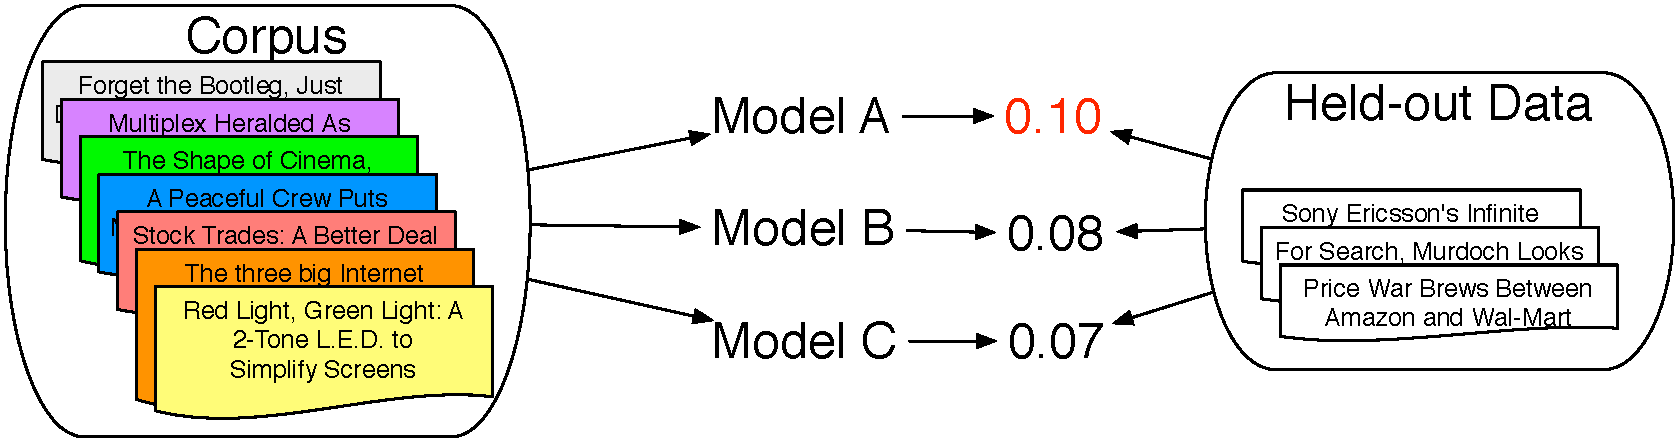
\includegraphics[width=\linewidth]{reading_tea_leaves/figures/heldout_4}  \\
	\large Measures predictive power, not what the topics are}
\end{center}

\begin{center}
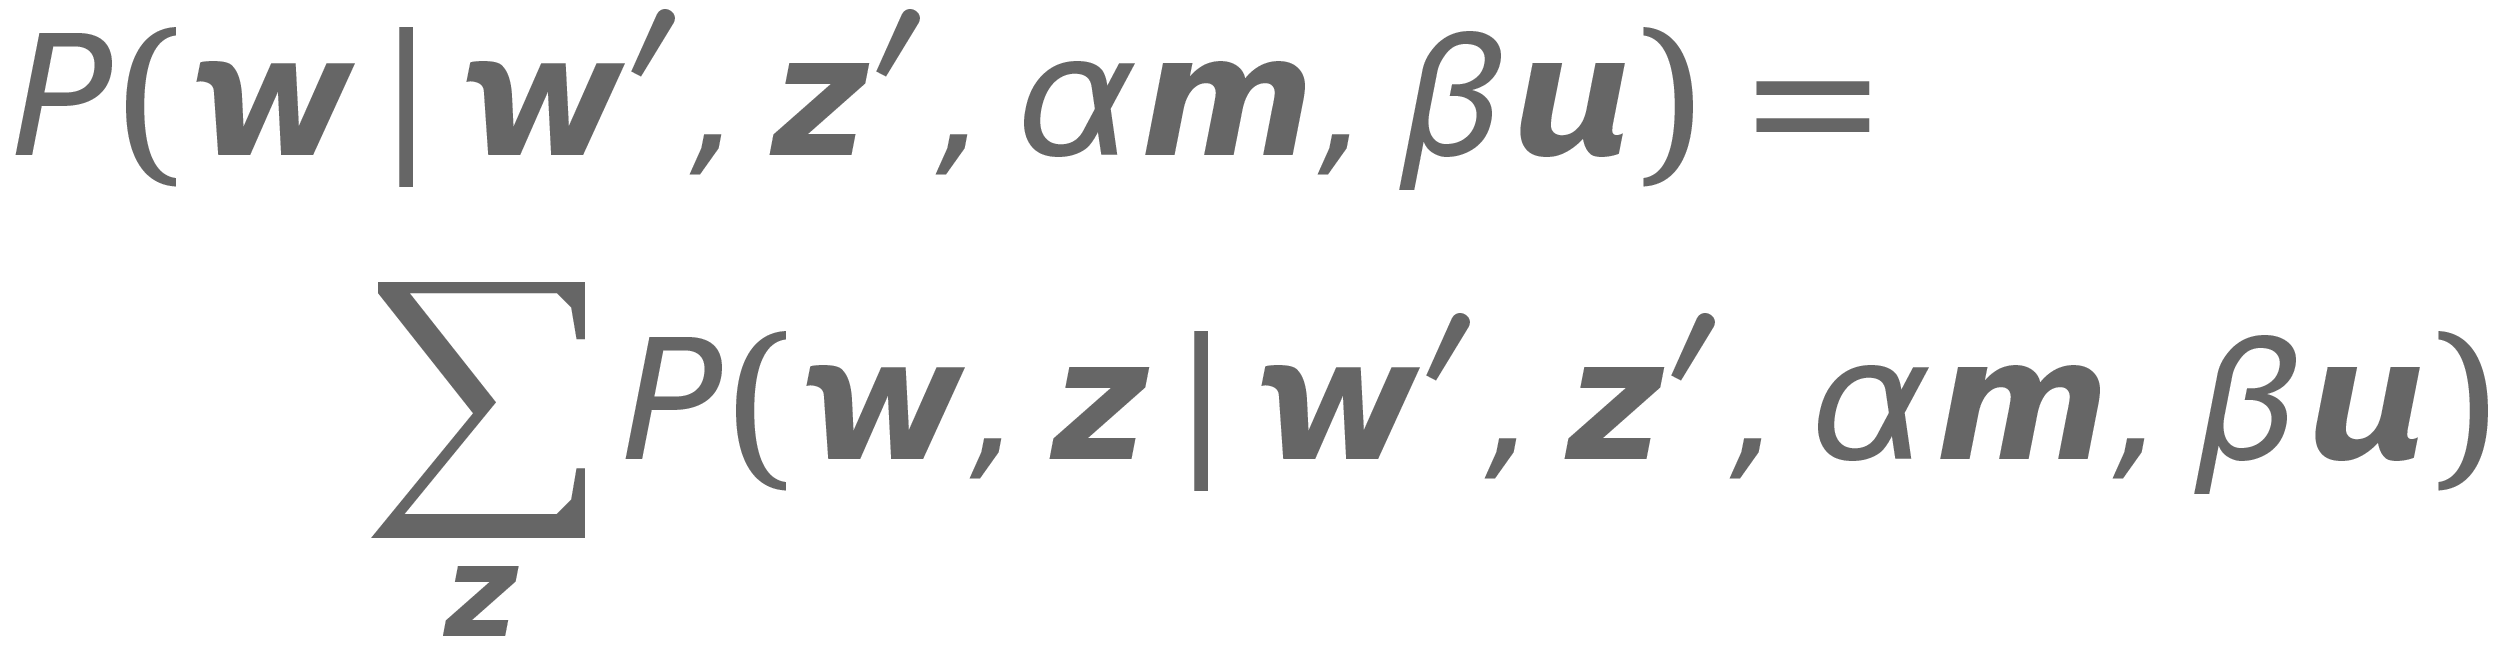
\includegraphics[width=0.5\linewidth]{topic_models/equations/evaluation} \\
How you compute it is important too~\cite{wallach-09b}
\end{center}

}

\frame{
  \frametitle{Word Intrusion}

  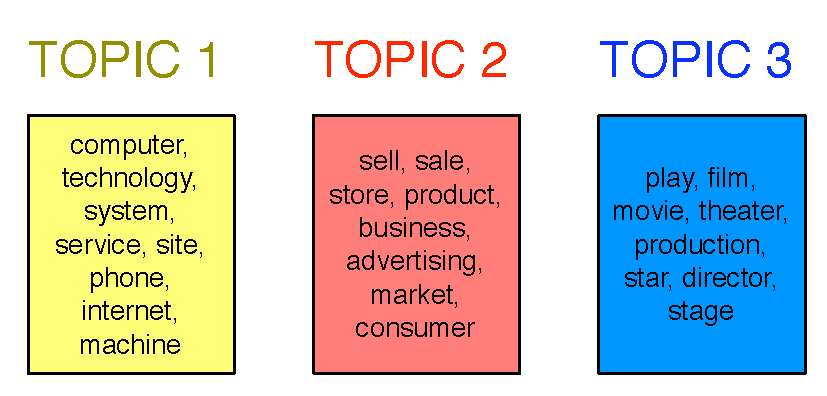
\includegraphics[width=\linewidth]{reading_tea_leaves/figures/nyt_topics_wide}
}


\frame{
  \frametitle{Word Intrusion}

  \begin{enumerate}
    \item Take the highest probability words from a topic

      \begin{block}{Original Topic}
        dog, cat, horse, pig, cow
      \end{block}
\pause
    \item Take a high-probability word from another topic and add it
      \begin{block}{Topic with Intruder}
        dog, cat, \alert<2->{apple}, horse, pig, cow
      \end{block}
\pause
     \item We ask users to find the word that doesn't belong
  \end{enumerate}
\begin{block}{Hypothesis}
If the topics are interpretable, users will consistently choose true intruder
\end{block}
}

\frame{
\frametitle{Word Intrusion}
\begin{center}
\only<1>{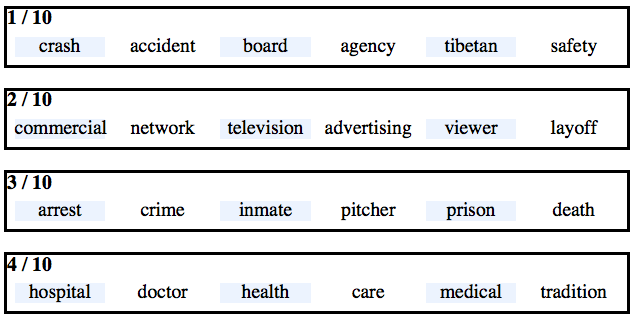
\includegraphics[width=\linewidth]{reading_tea_leaves/tasks/word1}  }
\only<2>{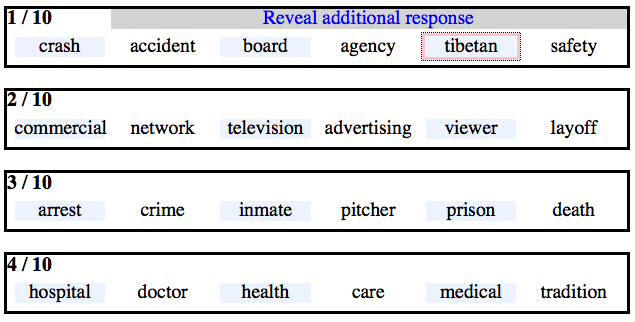
\includegraphics[width=\linewidth]{reading_tea_leaves/tasks/word2}  }
\pause
  \begin{itemize}
    \item Order of words was shuffled
    \item Which intruder was selected varied
    \item Model precision: percentage of users who clicked on intruder
  \end{itemize}

\end{center}
}

\frame{
\frametitle{Word Intrusion: Which Topics are Interpretable?}
  \begin{block}{New York Times, 50 LDA Topics}
    \begin{center}
      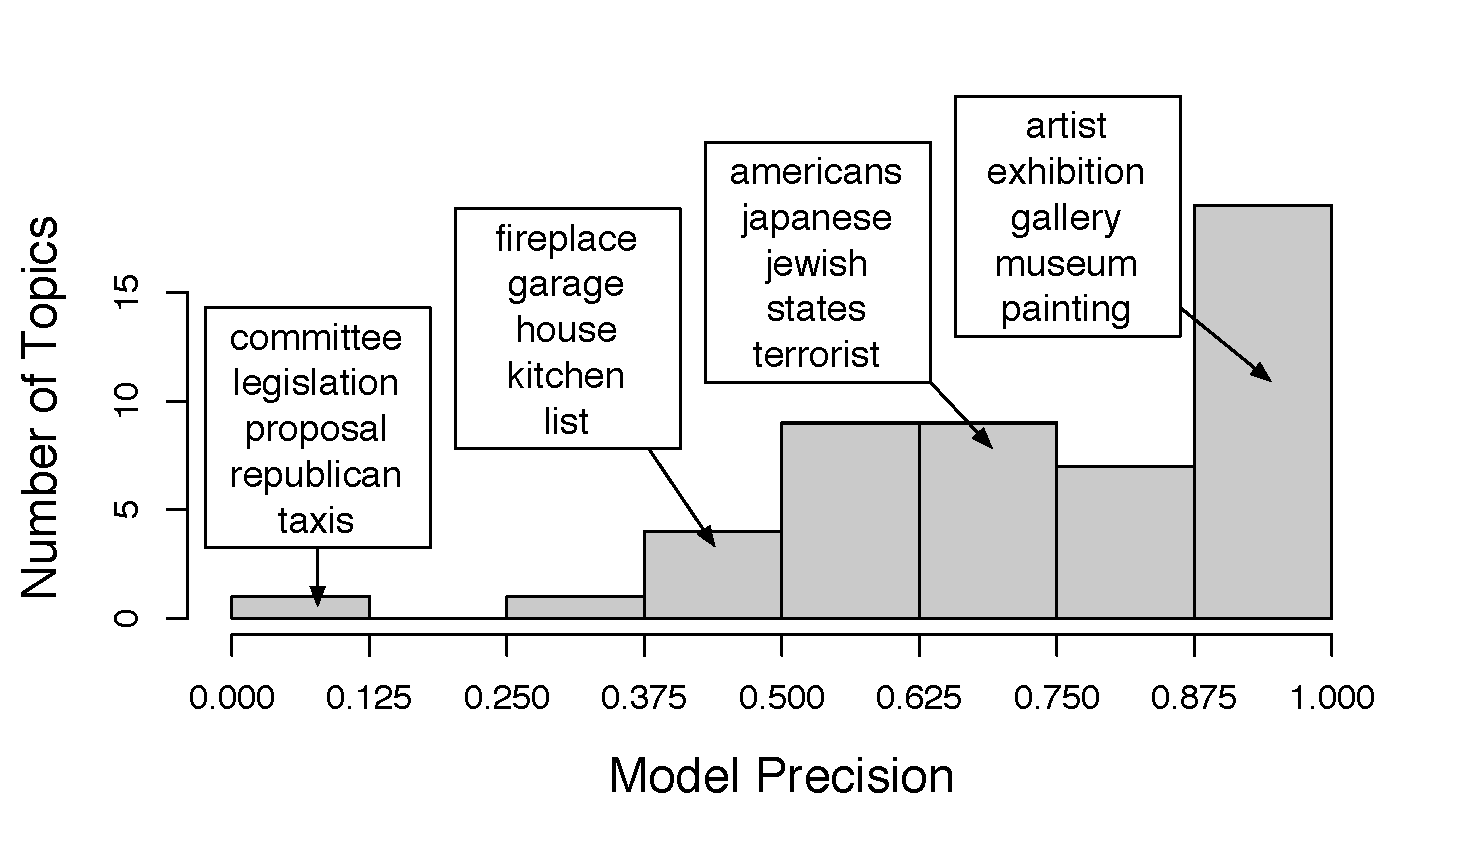
\includegraphics[width=0.8\linewidth]{reading_tea_leaves/figures/topic_precision}
    \end{center}
  \end{block}
  \begin{center}
    Model Precision: percentage of correct intruders found
  \end{center}
}



\frame{

\frametitle{Interpretability and Likelihood}
\begin{center}
\only<1>{Model Precision on New York Times}
\only<2>{Topic Log Odds on Wikipedia}
\end{center}

\begin{columns}
\column{.85\linewidth}
\begin{flushright}
  \only<1>{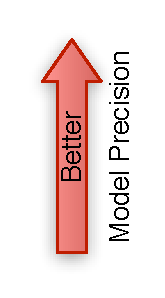
\includegraphics[scale=\graphscale]{reading_tea_leaves/tasks/mp}}
  \only<2>{
\includegraphics[scale=\graphscale]{reading_tea_leaves/tasks/tlo}}
  \only<1>{
\includegraphics[scale=\graphscale]{reading_tea_leaves/tasks/mp_y}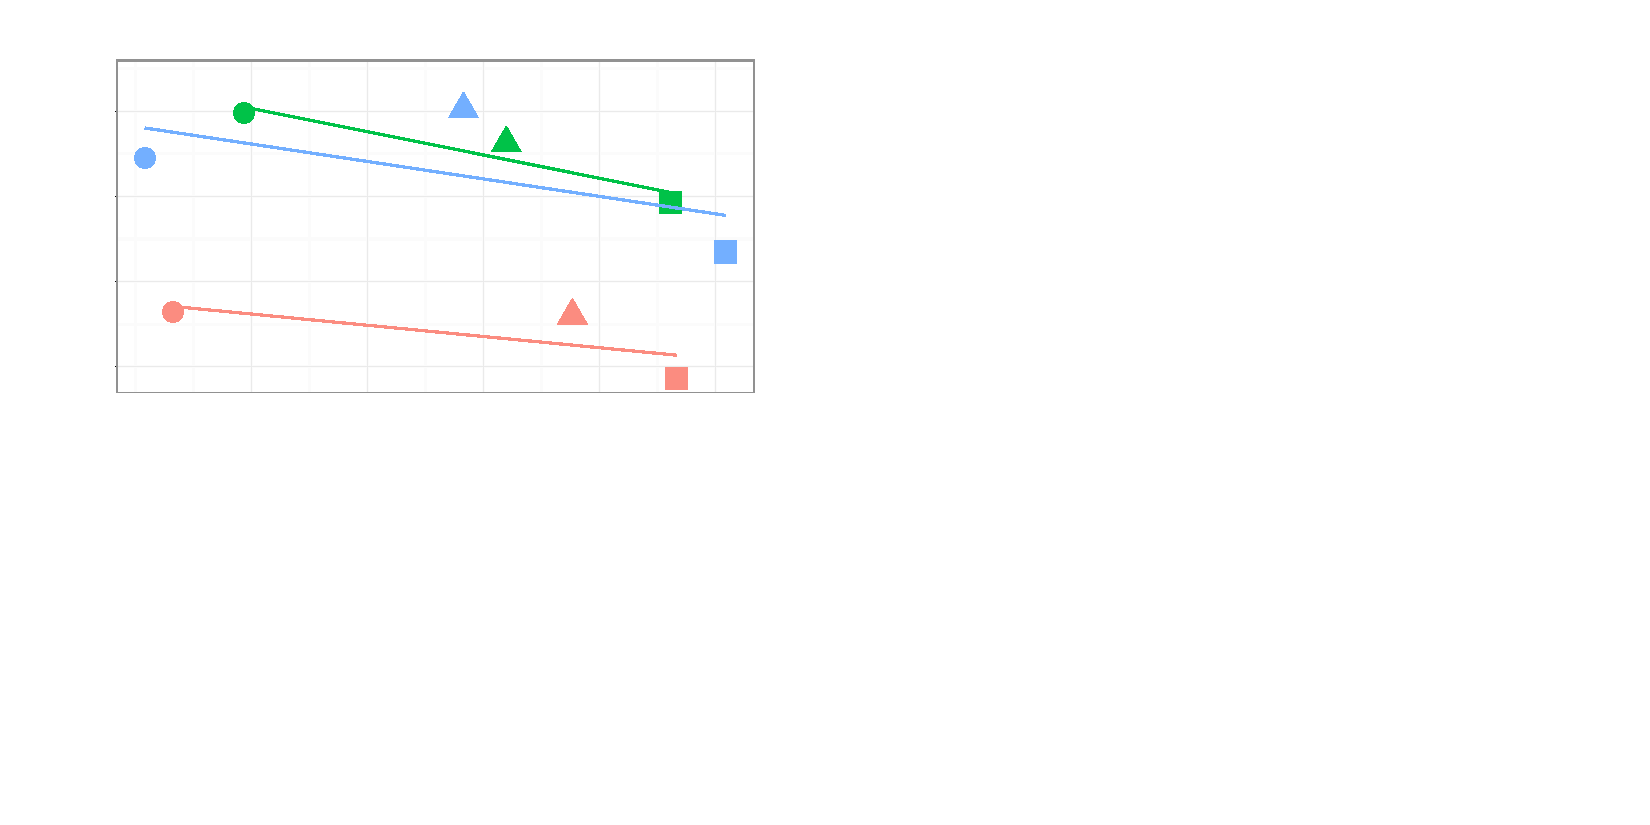
\includegraphics[scale=\graphscale]{reading_tea_leaves/tasks/nyt_mp}}
  \only<2>{
\includegraphics[scale=\graphscale]{reading_tea_leaves/tasks/tlo_y}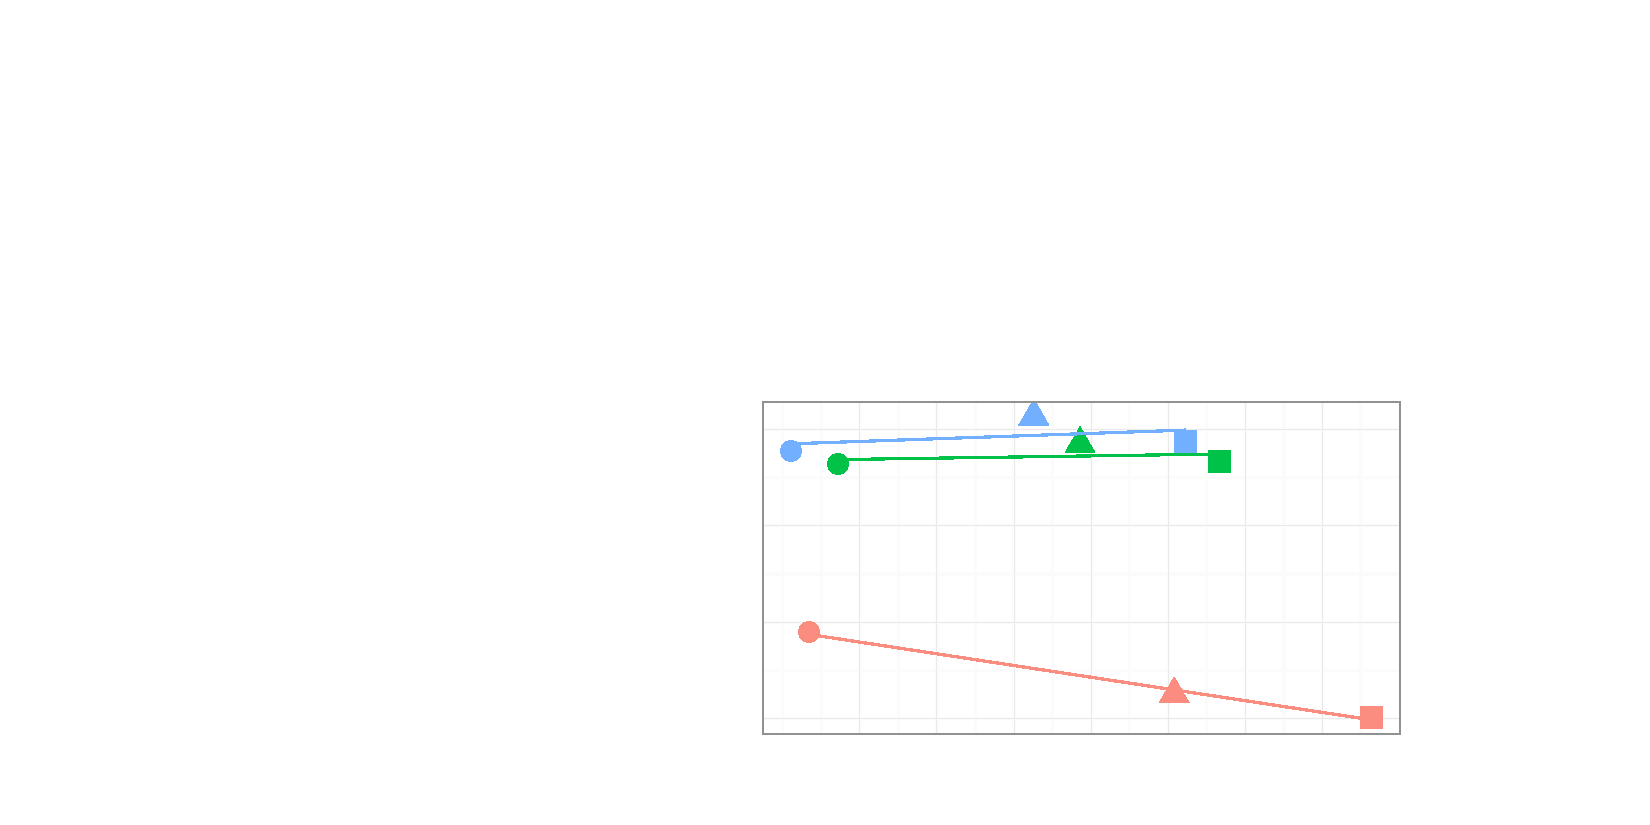
\includegraphics[scale=\graphscale]{reading_tea_leaves/tasks/wiki_tlo}} \\
  \only<1>{
\includegraphics[scale=\graphscale]{reading_tea_leaves/tasks/nyt_x}}
  \only<2>{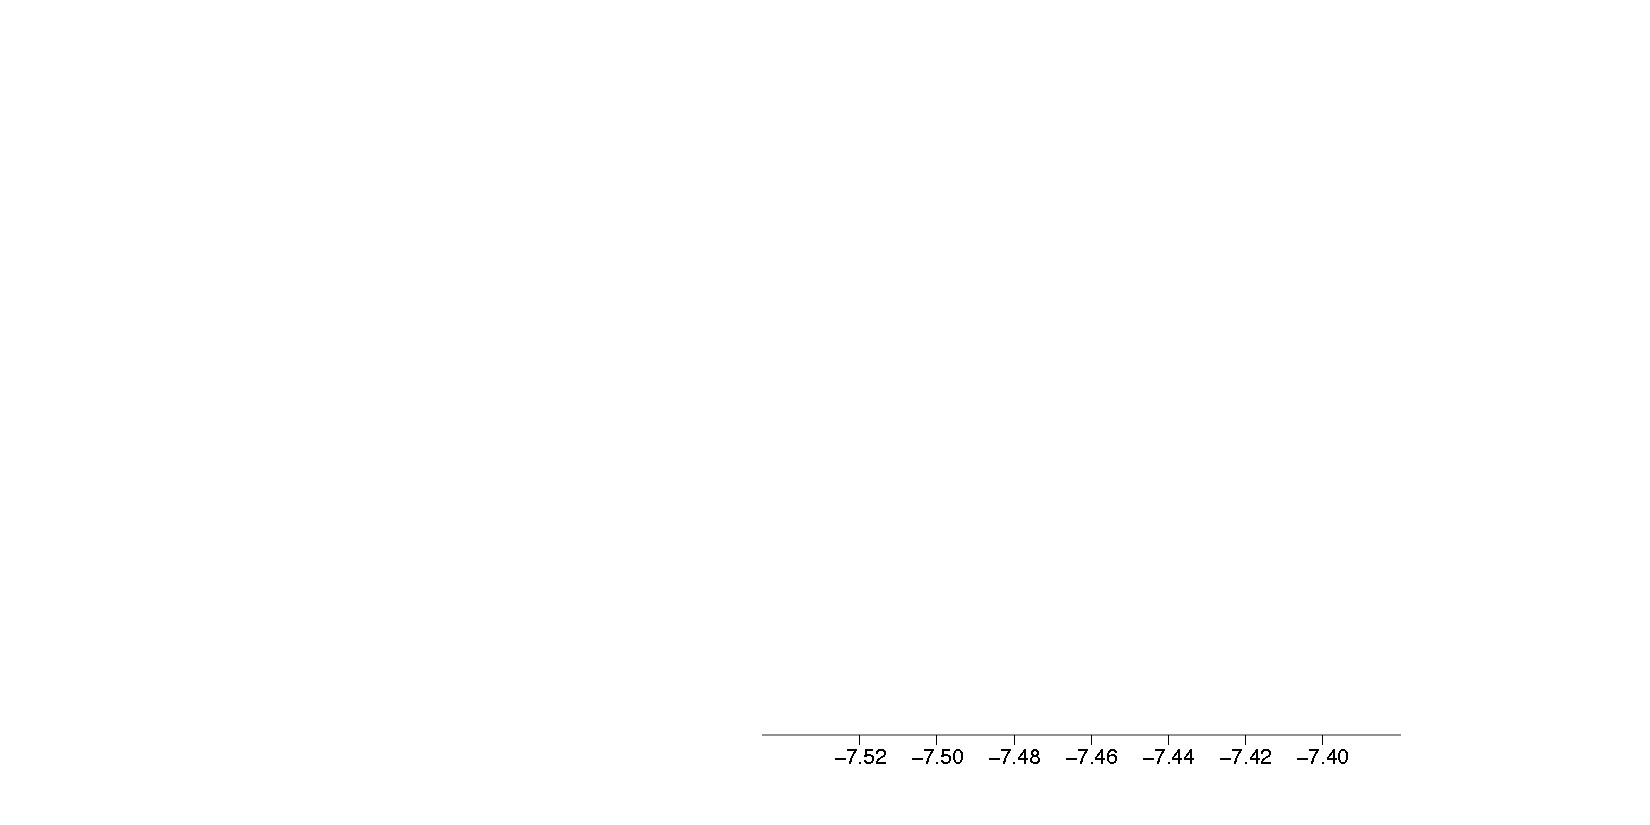
\includegraphics[scale=\graphscale]{reading_tea_leaves/tasks/wiki_x}}
\end{flushright}
\column{.15\linewidth}
  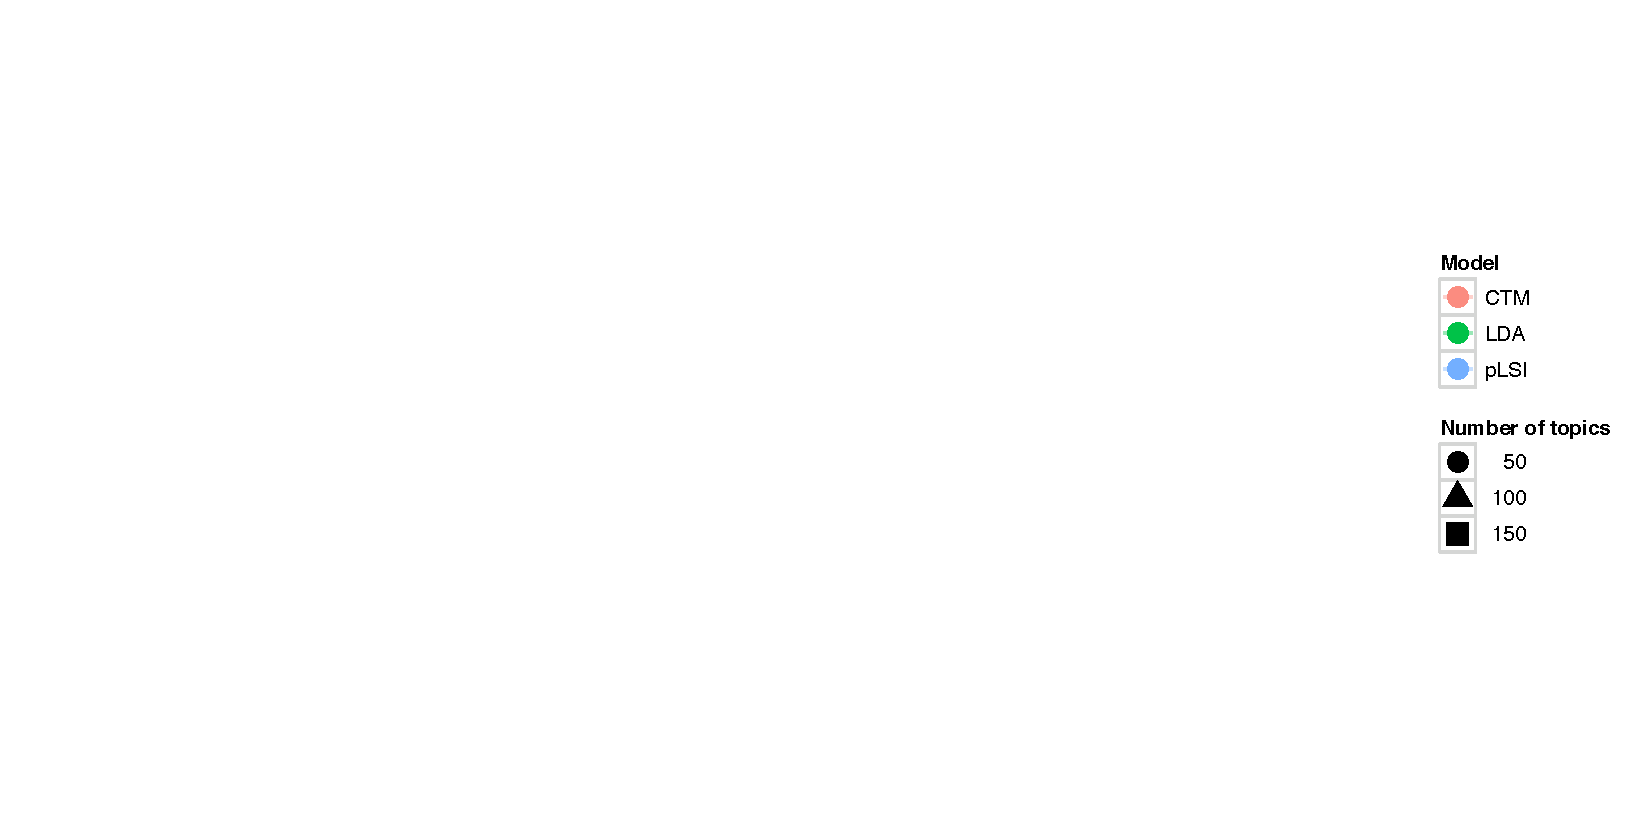
\includegraphics[scale=\graphscale]{reading_tea_leaves/tasks/legend}
\end{columns}
\vspace{-0.75cm}
\begin{center}
  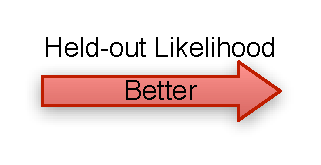
\includegraphics[scale=\graphscale]{reading_tea_leaves/tasks/held-out} \\
\only<1> {within a model, higher likelihood $\not =$ higher interpretability}
\only<2> {across models, higher likelihood $\not =$ higher interpretability}
\end{center}
}


\begin{frame}
  \frametitle{Evaluation Takeaway}

  \begin{itemize}
    \item Measure what you care about~\cite{chang-09c}
      \item If you care about prediction, likelihood is good
\item If you care about a particular task, measure that
    \end{itemize}

\end{frame}

\fi


\section{Inference}


\providecommand{\dirfunc}[3]{ \frac{ \prod_{#1}^{#2} \g{ #3 } } { \g{ \sum_{#1}^{#2} #3 }}}
\providecommand{\dirnum}[4]{ \frac{\g{ #3 }}{#4} \prod_{#1}^{#2} }
\providecommand{\dirden}[3]{ \g{ \sum_{#1}^{#2} #3 } }

\begin{frame}
\frametitle{Inference}

\begin{itemize}
\item We are interested in posterior distribution
\begin{equation}
p(Z | X, \Theta)
\end{equation}
\pause
\item Here, latent variables are topic assignments $z$ and topics $\theta$.  $X$ is the words (divided into documents), and $\Theta$ are hyperparameters to Dirichlet distributions: $\alpha$ for topic proportion, $\lambda$ for topics.
\begin{equation}
p({\bm z}, {\bm \beta}, {\bm \theta} | {\bm w}, \alpha, \lambda)
\end{equation}
\pause
\begin{align*}
p({\bm w}, {\bm z}, {\bm \theta}, {\bm \beta} & | \alpha, \lambda) = \\
& \prod_{k} p(\beta_k | \lambda) \prod_{d} p(\theta_d | \alpha) \prod_{n}
p(z_{d,n} | \theta_d) p(w_{d,n} | \beta_{z_{d,n}})
\end{align*}
\end{itemize}
\end{frame}



\begin{frame}
\frametitle{Gibbs Sampling}
\begin{itemize}
\item A form of Markov Chain Monte Carlo
\item Chain is a sequence of random variable states
\item Given a state $\{z_1, \dots z_N\}$ given certain technical conditions, drawing $z_k \sim p(z_1, \dots z_{k-1}, z_{k+1}, \dots z_N | X, \Theta)$ for all $k$ (repeatedly) results in a Markov Chain whose stationary distribution \emph{is} the posterior.
\item For notational convenience, call ${\bm z}$ with $z_{d,n}$ removed ${\bm z}_{-d,n}$
\end{itemize}
\end{frame}

\frame{
	\frametitle{Inference}
	\begin{center}
\only<1> {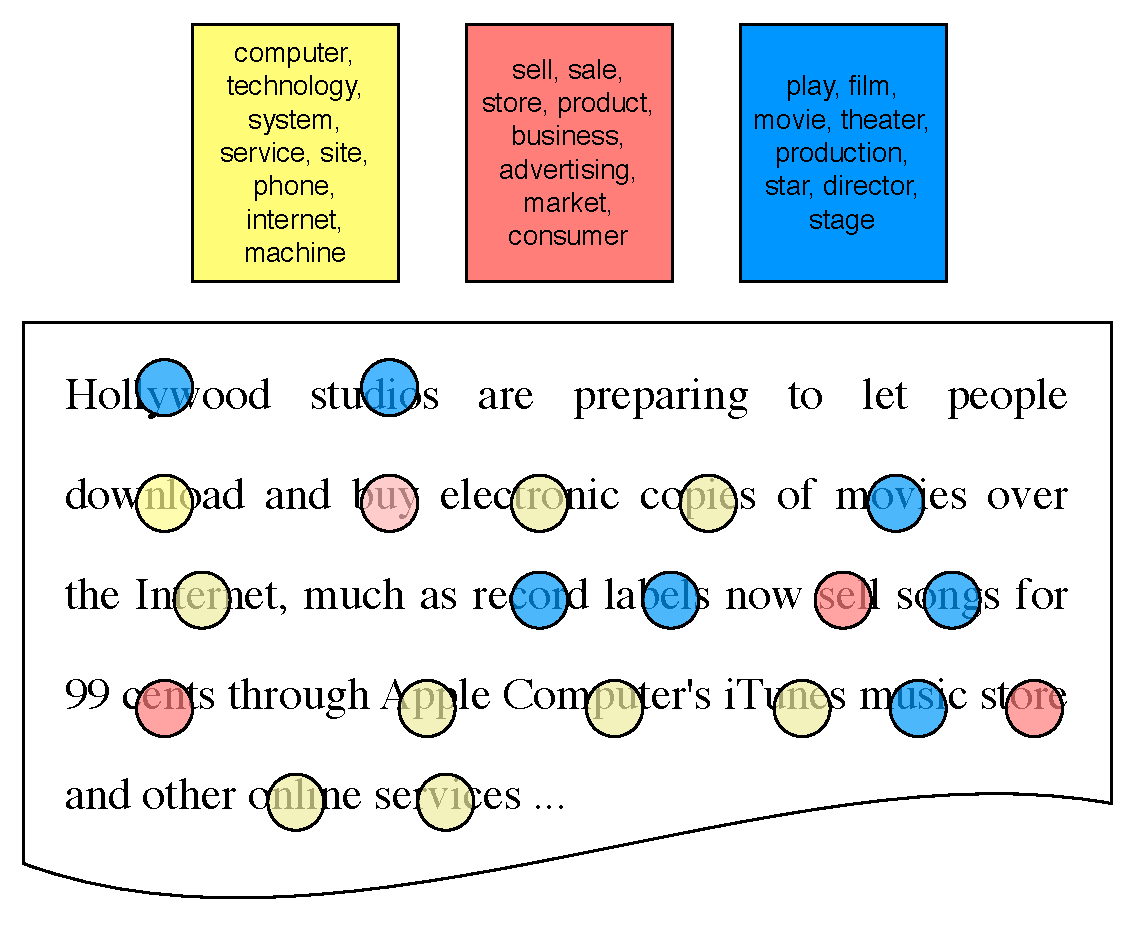
\includegraphics[width=.8\linewidth]{topic_models/inference_3}}
\only<2> {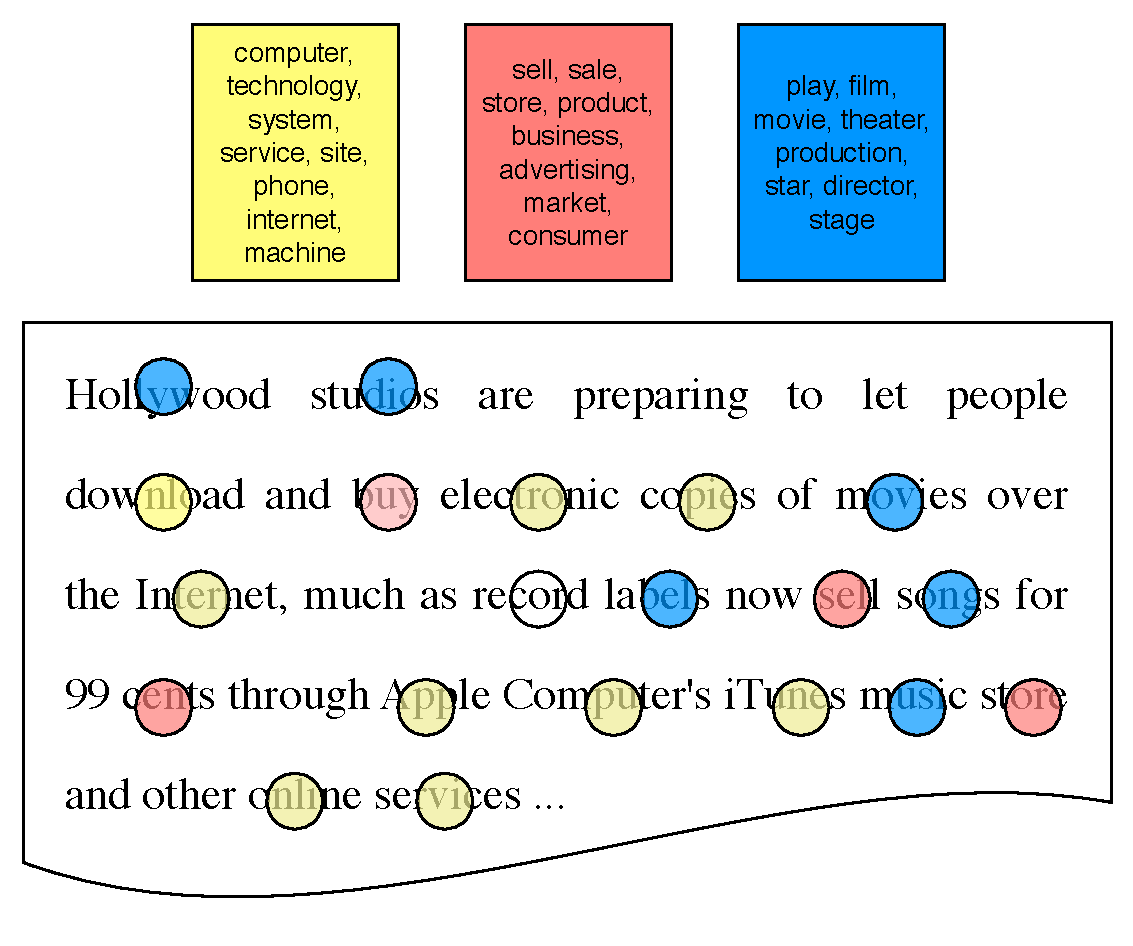
\includegraphics[width=.8\linewidth]{topic_models/inference_4}}
\only<3> {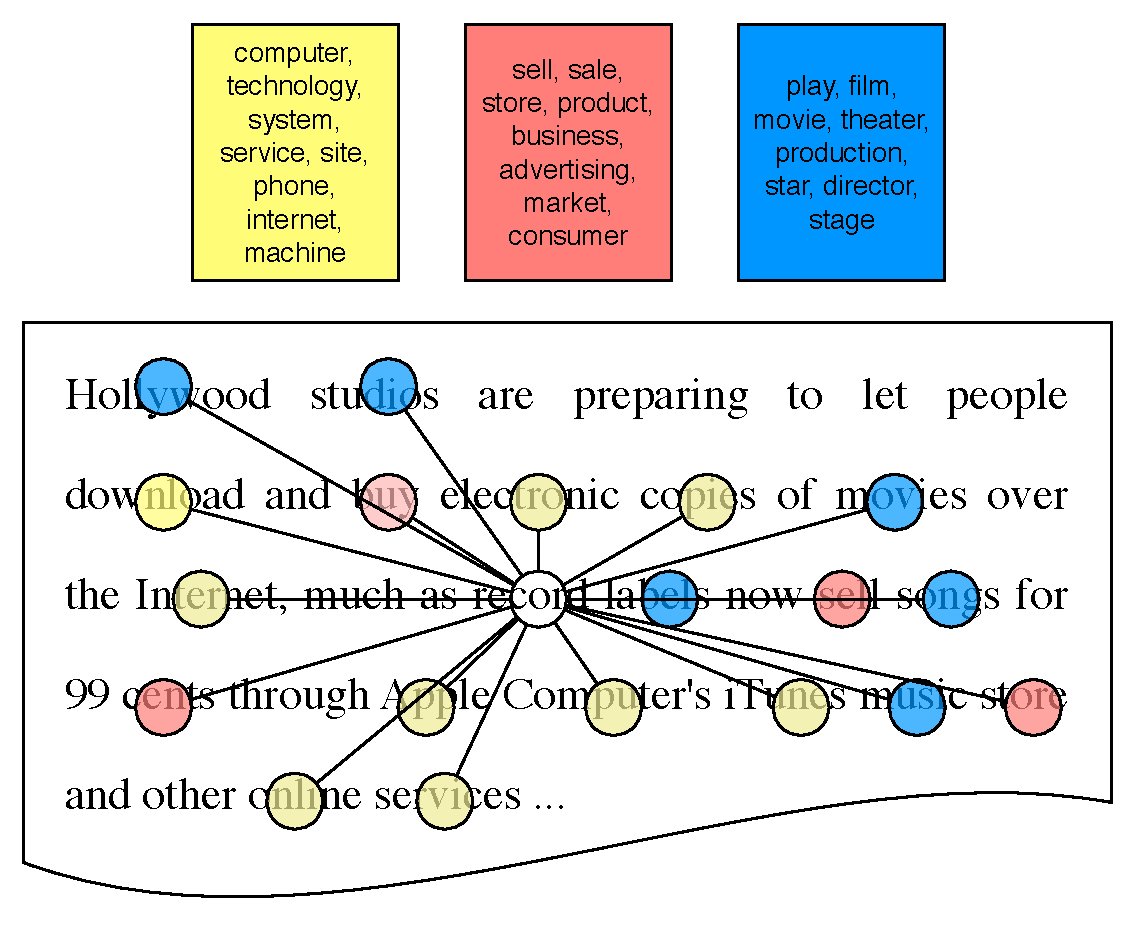
\includegraphics[width=.8\linewidth]{topic_models/inference_5}}
\only<4> {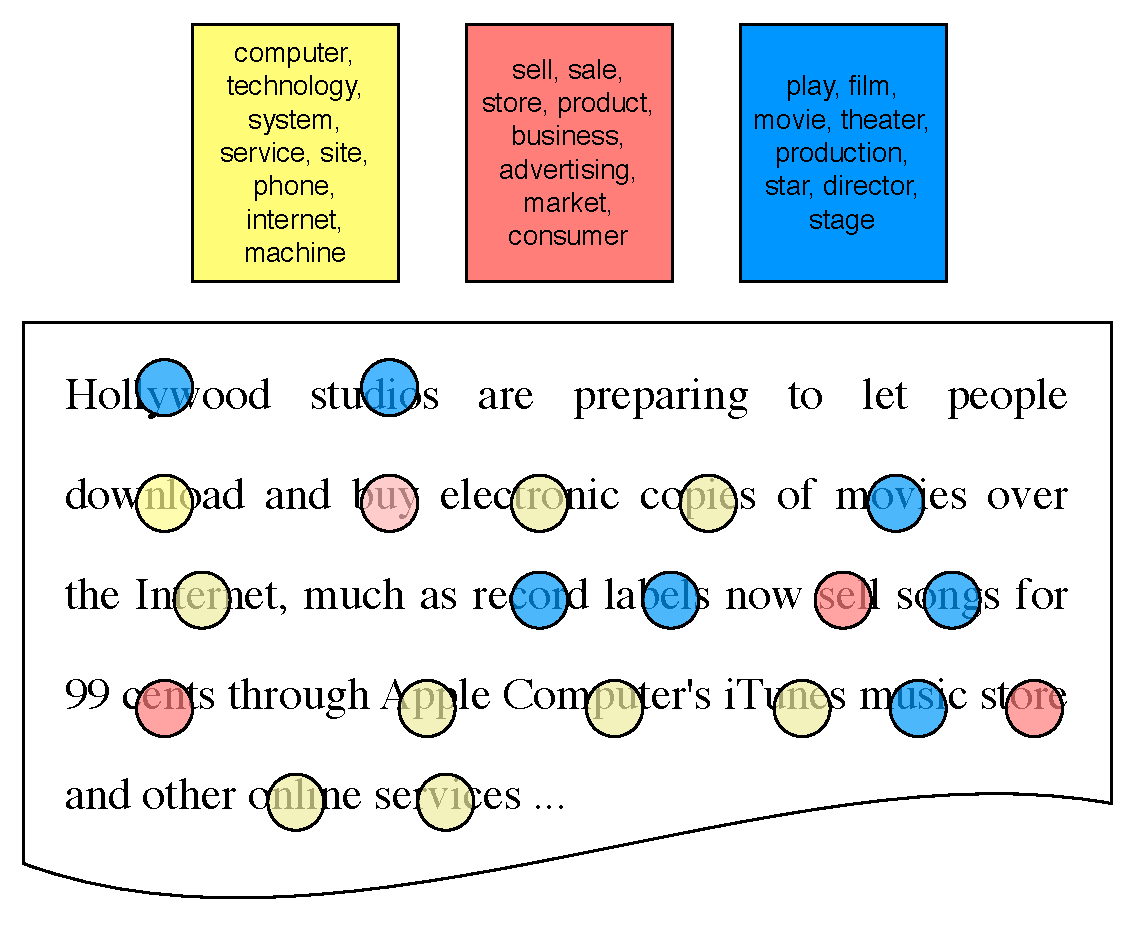
\includegraphics[width=.8\linewidth]{topic_models/inference_3}}
\only<5> {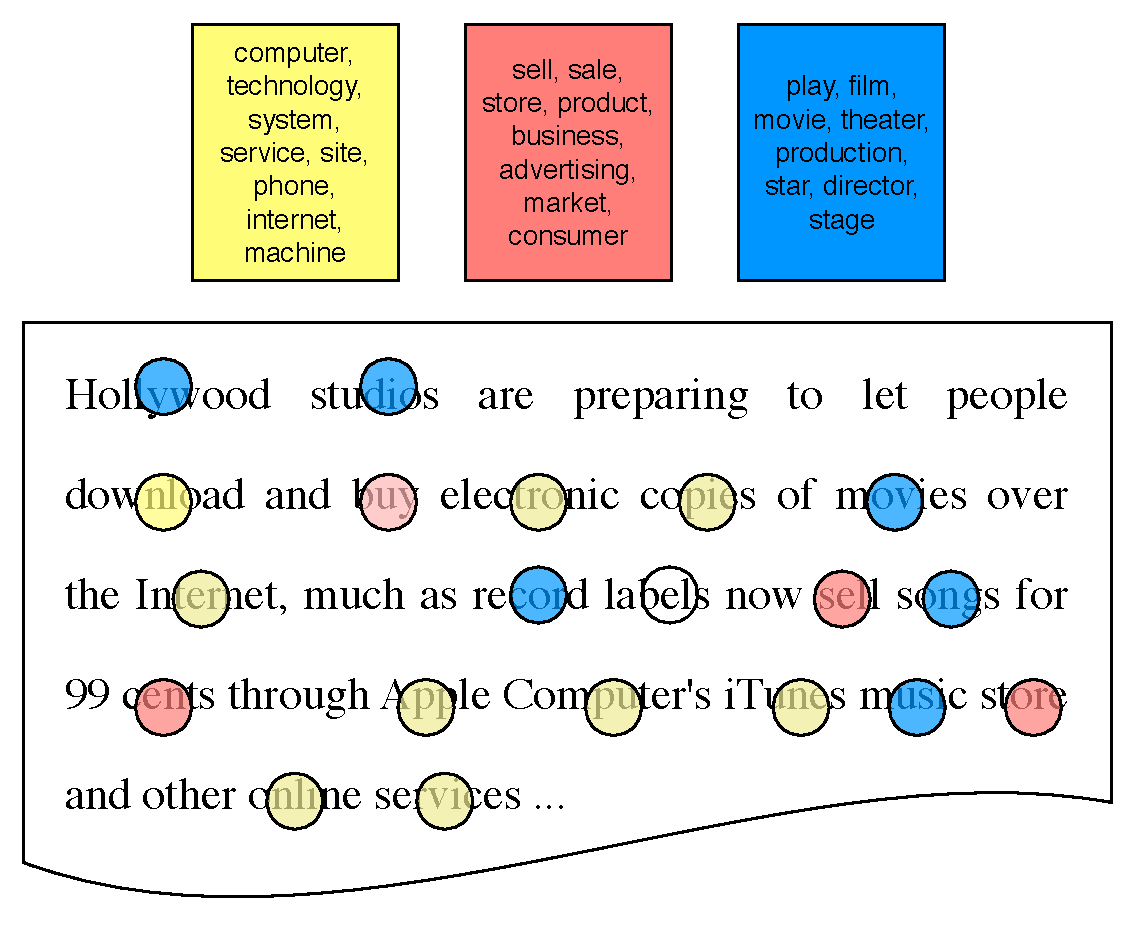
\includegraphics[width=.8\linewidth]{topic_models/inference_6}}
\only<6> {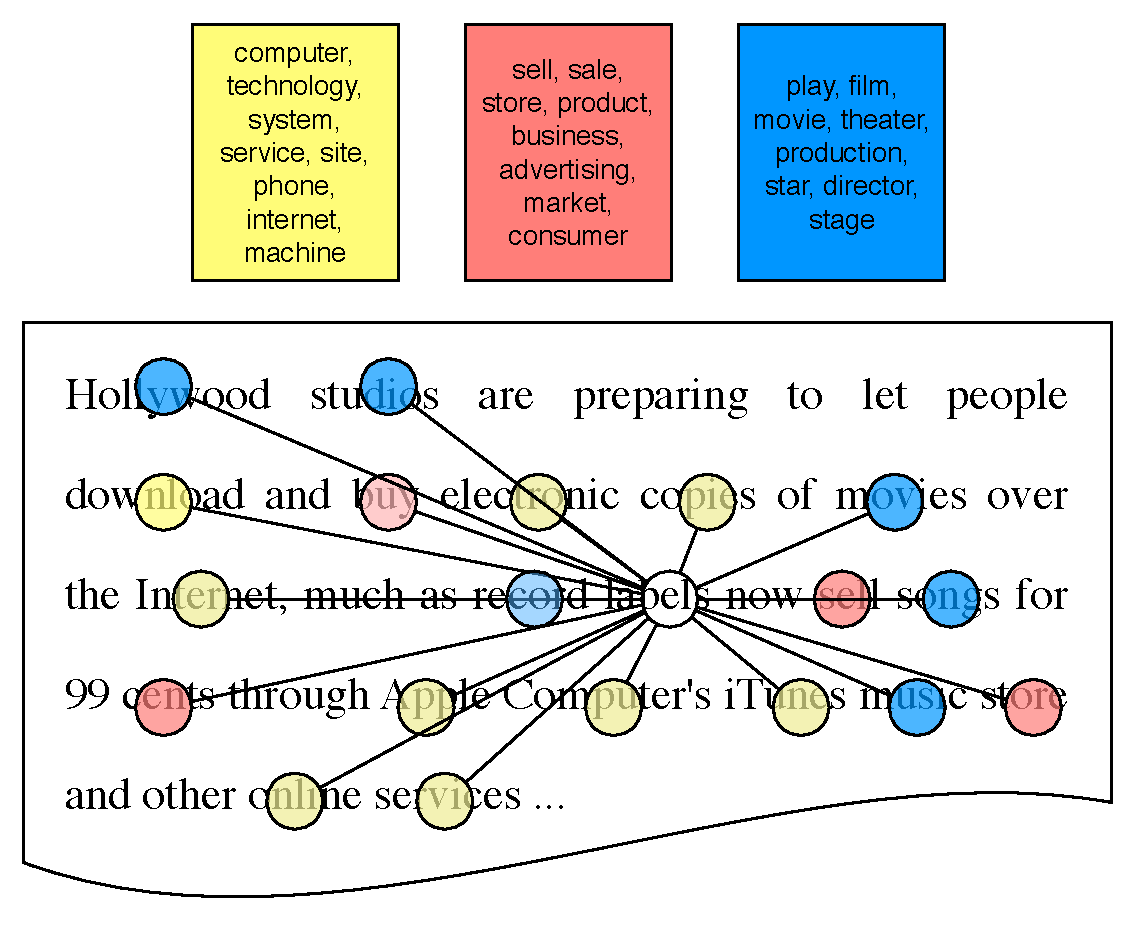
\includegraphics[width=.8\linewidth]{topic_models/inference_7}}
\only<7> {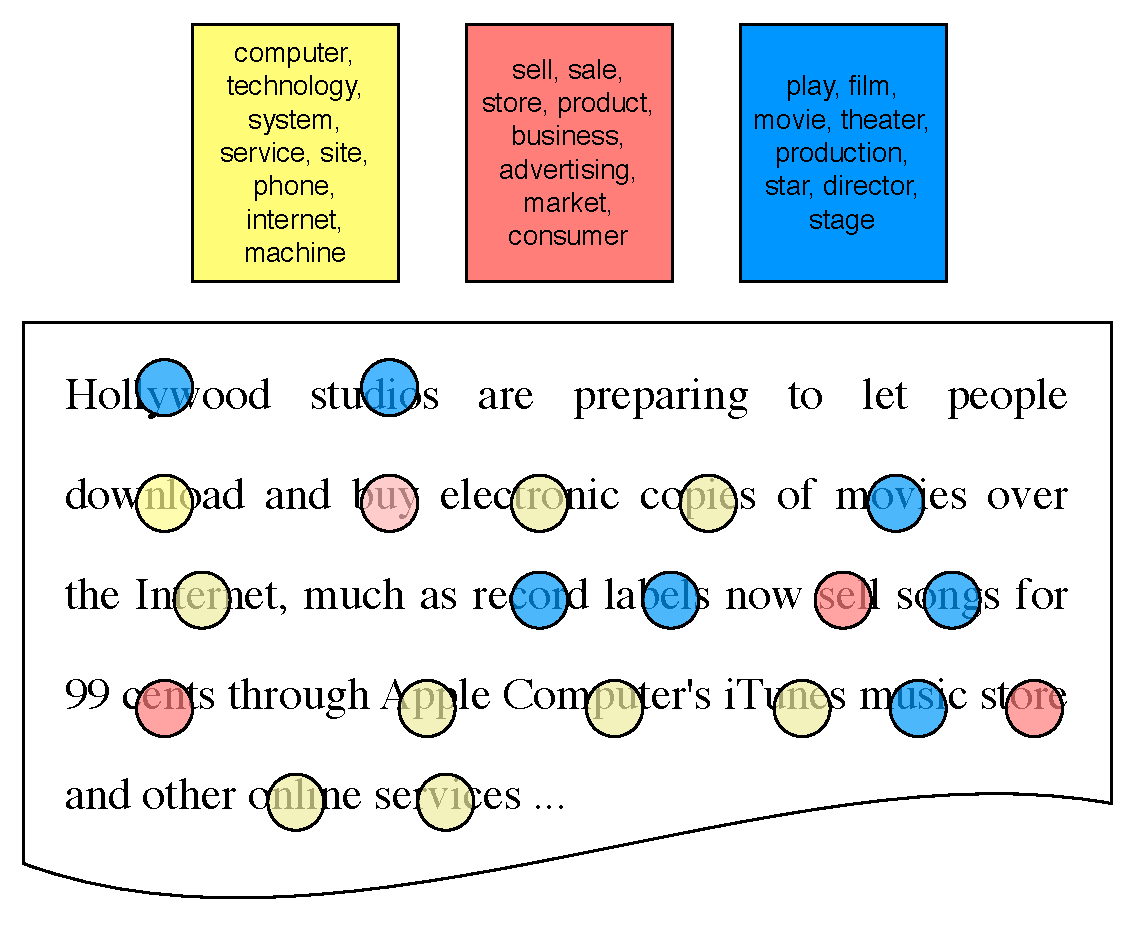
\includegraphics[width=.8\linewidth]{topic_models/inference_3}}
	\end{center}
}


\ifconjugacy

\begin{frame}
\frametitle{Gibbs Sampling}
\begin{itemize}
\item For LDA, we will sample the topic assignments
\item Thus, we want:
\begin{equation*}
p(z_{d,n} = k | {\bm z}_{-d,n}, {\bm w}, \alpha, \lambda) = \frac{ p(z_{d,n} = k, {\bm z}_{-d,n} | {\bm w}, \alpha, \lambda)} { p({\bm z}_{-d,n} | {\bm w},\alpha, \lambda)}
\end{equation*}
\pause
\item The topics and per-document topic proportions are integrated out / marginalized
\item Let $n_{d,i}$ be the number of words taking topic $i$ in document $d$.  Let $v_{k,w}$ be the number of times word $w$ is used in topic $k$.
\end{itemize}


\begin{equation*}
= \frac{ \int_{\theta_d} \left( \prod_{i \not = k} \theta_d^{\alpha_i + n_{d,i} - 1} \right)\theta_d^{\alpha_k + n_{d,i} } d\theta_d \int_{\beta_{k}}    \left( \prod_{i \not = w_{d,n}} \beta_{k,i} ^{ \lambda_i + v_{k,i} - 1} \right) \beta_{k, w_{d,n}}^{\lambda_i + v_{k,i}} d\beta_k } { \int_{\theta_d} \left( \prod_{i} \theta_d^{\alpha_i + n_{d,i} - 1} \right) d\theta_d \int_{\beta_{k}}    \left( \prod_{i} \beta_{k,i} ^{ \lambda_i + v_{k,i} - 1} \right) d\beta_k }
\end{equation*}
\end{frame}

\else

\begin{frame}
\frametitle{Gibbs Sampling}
\begin{itemize}
\item For LDA, we will sample the topic assignments
\item The topics and per-document topic proportions are integrated out / marginalized / Rao-Blackwellized
\item Thus, we want:
\begin{equation*}
p(z_{d,n} = k | {\bm z}_{-d,n}, {\bm w}, \alpha, \lambda) = \frac{n_{d, k} + \alpha_k}{ \sum_{i}^{K} { n_{d,i} + \alpha_i}} \frac{v_{k, w_{d,n}} + \lambda_{w_{d,n}}}{ \sum_{i} { v_{k,i} + \lambda_{i} }}
\end{equation*}
\end{itemize}
\end{frame}

\fi



\ifconjugacy

\begin{frame}
\frametitle{Gibbs Sampling}
\begin{itemize}
\item Integral is normalizer of Dirichlet distribution
\begin{equation*}
\int_{\beta_{k}}    \left( \prod_{i} \beta_{k,i} ^{ \lambda_i + v_{k,i} - 1} \right) d\beta_k = \dirfunc{i}{V}{\beta_i + v_{k,i}}
\end{equation*}
\pause
\item So we can simplify
\end{itemize}
\begin{footnotesize}
\begin{align*}
& \frac{ \int_{\theta_d} \left( \prod_{i \not = k} \theta_d^{\alpha_i + n_{d,i}
      - 1} \right)\theta_d^{\alpha_k + n_{d,i} } d\theta_d \int_{\beta_{k}}
  \left( \prod_{i \not = w_{d,n}} \beta_{k,i} ^{ \lambda_i + v_{k,i} - 1}
  \right) \beta_{k, w_{d,n}}^{\lambda_i + v_{k,i}} d\beta_k } { \int_{\theta_d}
  \left( \prod_{i} \theta_d^{\alpha_i + n_{d,i} - 1} \right) d\theta_d
  \int_{\beta_{k}}    \left( \prod_{i} \beta_{k,i} ^{ \lambda_i + v_{k,i} - 1}
  \right) d\beta_k } = \\
& \frac{
  \dirnum{i \not = k}{K}{\alpha_k + n_{d,k} + 1}{ \g{\sum_{i}^{K} \alpha_i +
      n_{d,i} + 1} } \g{\alpha_k + n_{d,k}}  }
{ \dirfunc{i}{K}{\alpha_i + n_{d,i}} }
% -----------------------------------
\frac{
 \dirnum{i \not = w_{d,n}}{V}{\lambda_{w_{d,n}} + v_{k,w_{d,n}} + 1}{ \g{\sum_{i}^{V} \lambda_i + v_{k,i} + 1} } \g{\lambda_k + v_{k,w_{d,n}}}
}{ \dirfunc{i}{V}{\lambda_i + v_{k,i}} } \\
% -----------------------------------
\end{align*}
\end{footnotesize}
\end{frame}


\begin{frame}

\begin{block}{Gamma Function Identity}
	\begin{equation}
		z = \frac{\Gamma(z + 1)}{\Gamma(z)}
	\end{equation}
\end{block}

\begin{footnotesize}
\begin{align*}
& \frac{
  \dirnum{i \not = k}{K}{\alpha_k + n_{d,k} + 1}{ \g{\sum_{i}^{K} \alpha_i +
      n_{d,i} + 1} } \g{\alpha_k + n_{d,k}}  }
{ \dirfunc{i}{K}{\alpha_i + n_{d,i}} }
% -----------------------------------
\frac{
 \dirnum{i \not = w_{d,n}}{V}{\lambda_{w_{d,n}} + v_{k,w_{d,n}} + 1}{ \g{\sum_{i}^{V} \lambda_i + v_{k,i} + 1} } \g{\lambda_k + v_{k,w_{d,n}}}
}{ \dirfunc{i}{V}{\lambda_i + v_{k,i}} } \\
% -----------------------------------
& = \frac{n_{d, k} + \alpha_k}{ \sum_{i}^{K} { n_{d,i} + \alpha_i}} \frac{v_{k, w_{d,n}} + \lambda_{w_{d,n}}}{ \sum_{i} { v_{k,i} + \lambda_{i} }}
\end{align*}
\end{footnotesize}

\end{frame}
\else
\fi

\begin{frame}{Gibbs Sampling Equation}
  
\begin{equation}
\alert<5>{\frac{\alert<1>{n_{d, k}} +  \alert<3>{\alpha_k}}{ \sum_{i}^{K} { n_{d,i} +\alpha_i}}} \alert<6>{\frac{\alert<2>{v_{k, w_{d,n}}} + \alert<4>{\lambda_{w_{d,n}}}}{ \sum_{i} { v_{k,i} + \lambda_{i} }}}
\end{equation}

\begin{itemize}
  \item \alert<1>{Number of times document $d$ uses topic $k$}
  \item \alert<2>{Number of times topic $k$ uses word type $w_{d,n}$}
  \item \alert<3>{Dirichlet parameter for document to topic
      distribution}
  \item \alert<4>{Dirichlet parameter for topic to word distribution}
  \item \alert<5>{How much this document likes topic $k$}
  \item \alert<6>{How much this topic likes word $w_{d,n}$}
\end{itemize}

\end{frame}

\begin{frame}
  \frametitle{Sample Document}
    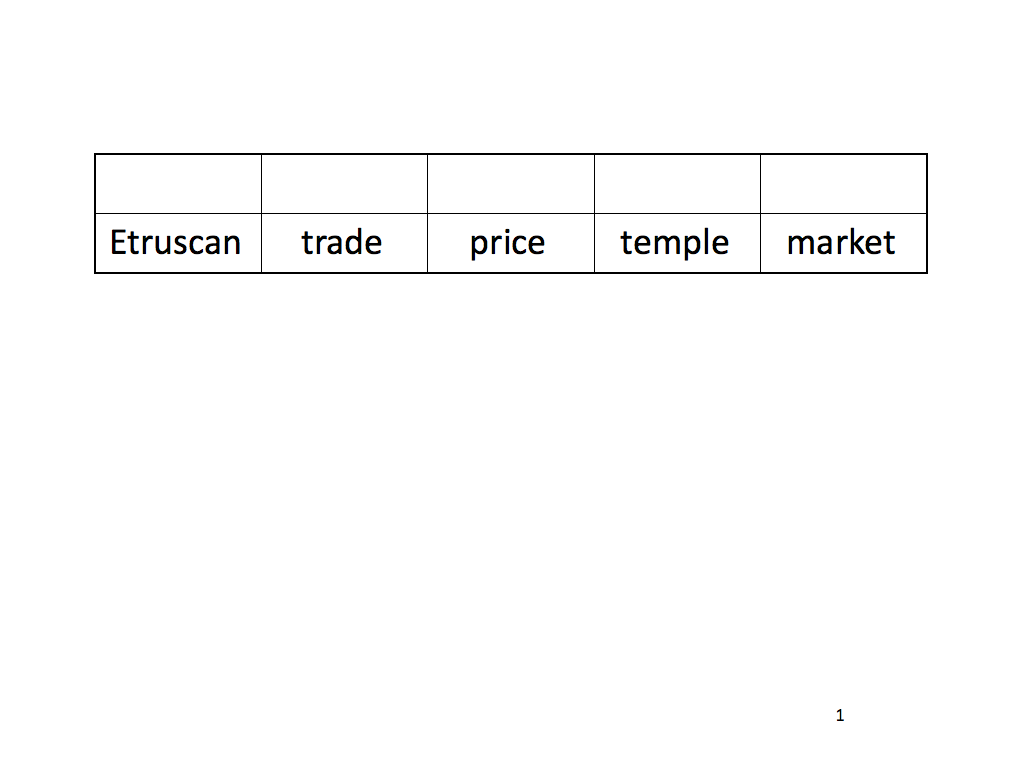
\includegraphics[width=\linewidth]{topic_models/mimno_001}
\end{frame}

\begin{frame}
  \frametitle{Sample Document}
    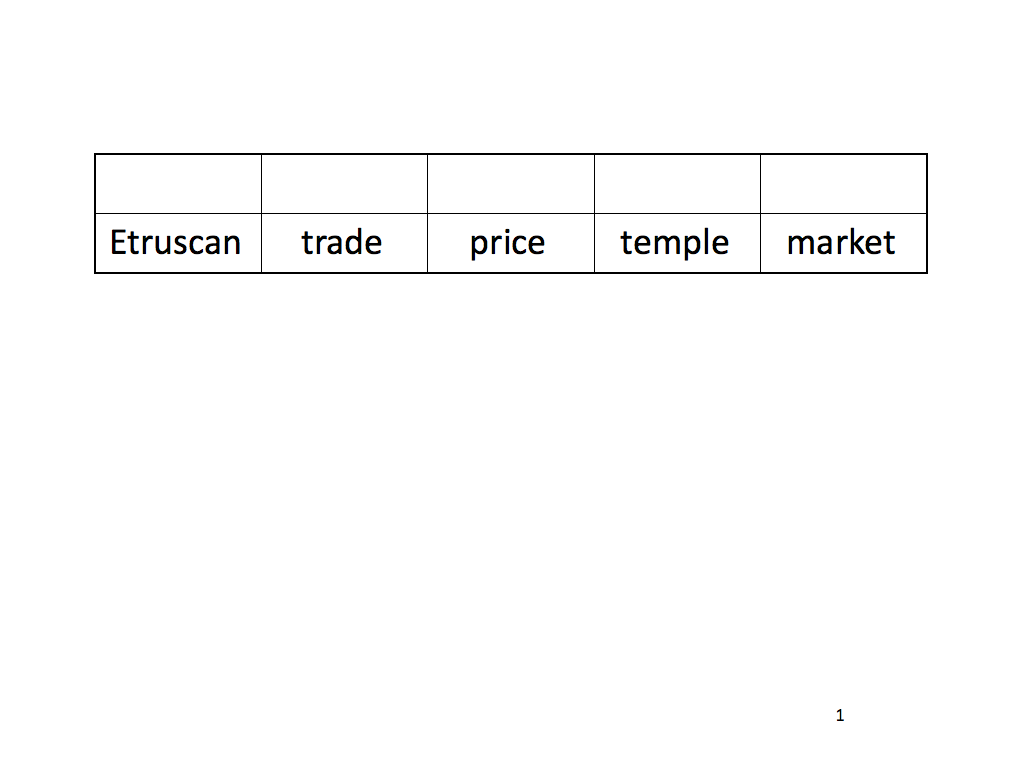
\includegraphics[width=\linewidth]{topic_models/mimno_001}
\end{frame}

\begin{frame}
  \frametitle{Randomly Assign Topics}
    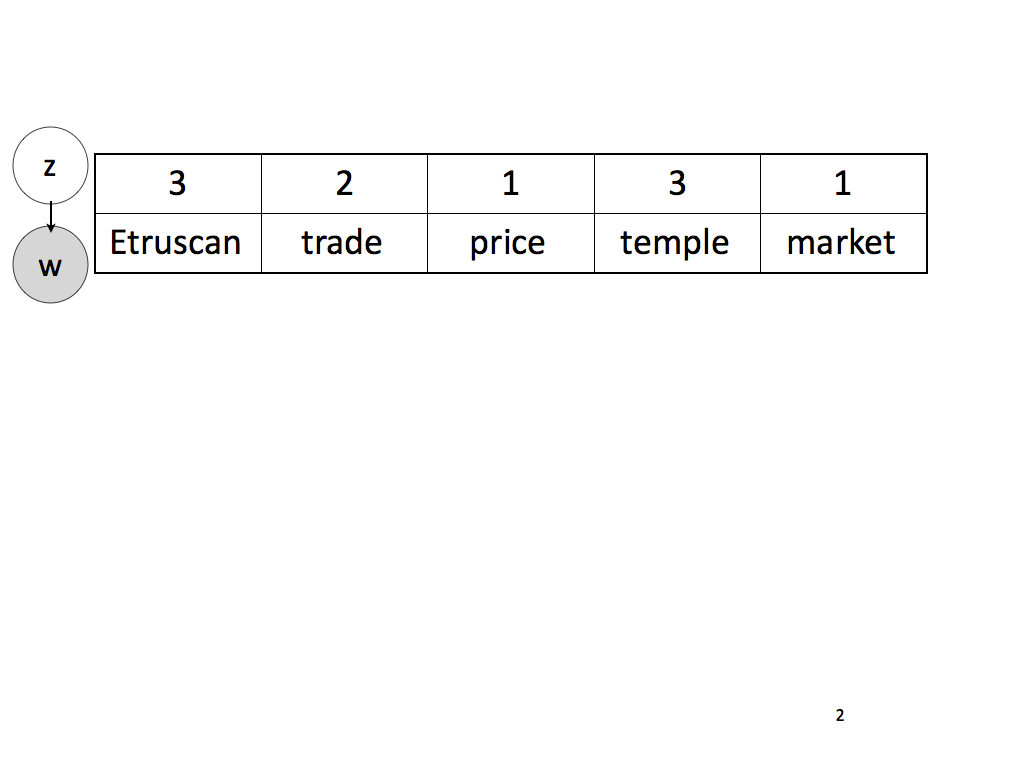
\includegraphics[width=\linewidth]{topic_models/mimno_002}
\end{frame}

\begin{frame}
  \frametitle{Randomly Assign Topics}
    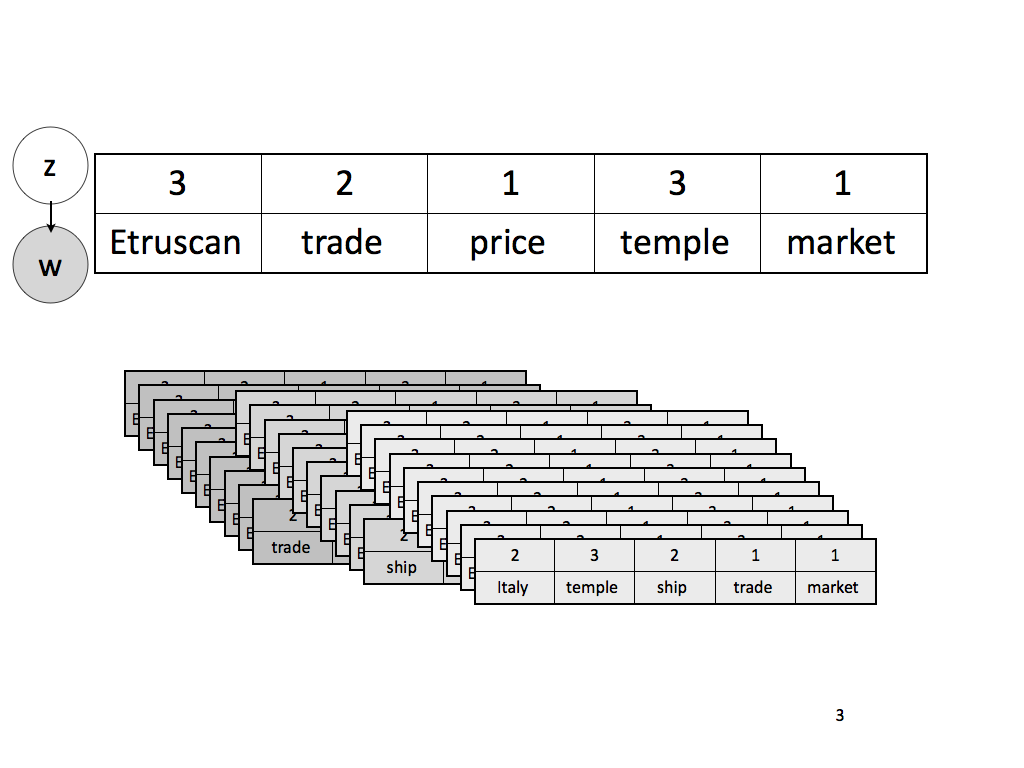
\includegraphics[width=\linewidth]{topic_models/mimno_003}
\end{frame}

\begin{frame}
  \frametitle{Total Topic Counts}
    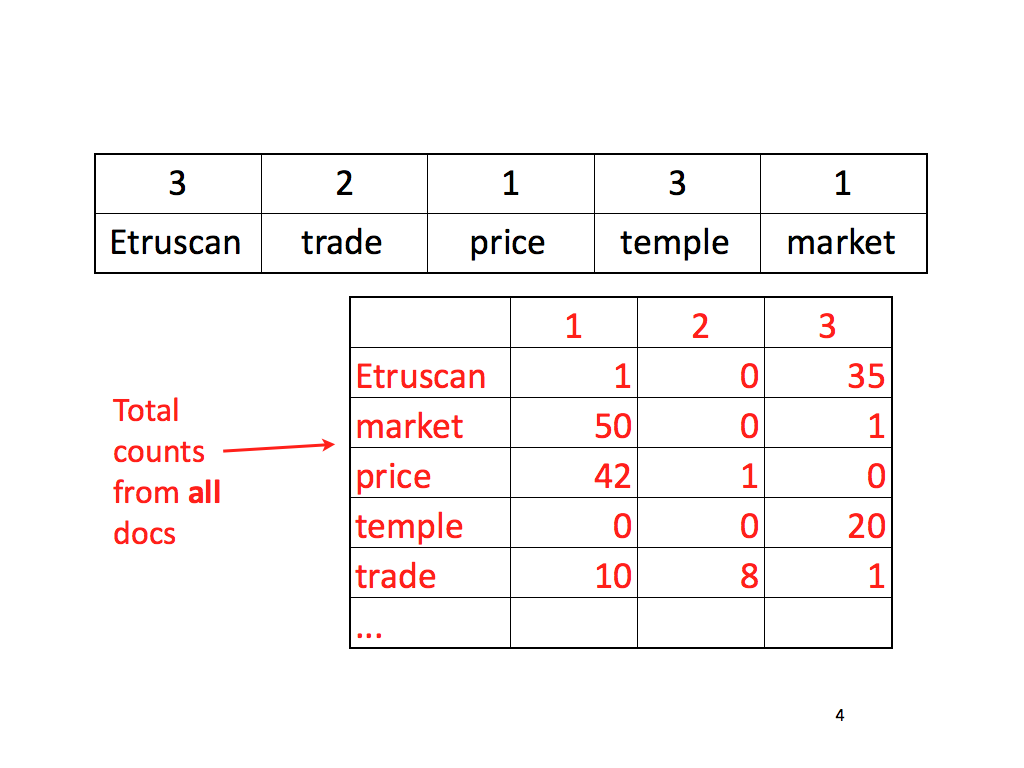
\includegraphics[width=\linewidth]{topic_models/mimno_004}

\pause

\vspace{-3cm}

\begin{block}{Sampling Equation}
	\begin{equation*}
          \frac{n_{d, k} + \alpha_k}{ \sum_{i}^{K} { n_{d,i} + \alpha_i}} \frac{\alert<3>{v_{k, w_{d,n}}} + \lambda_{w_{d,n}}}{ \sum_{i} { \alert<3>{v_{k,i}} + \lambda_{i} }}
	\end{equation*}
\end{block}

\end{frame}


\begin{frame}
  \frametitle{We want to sample this word \dots}
    \only<1>{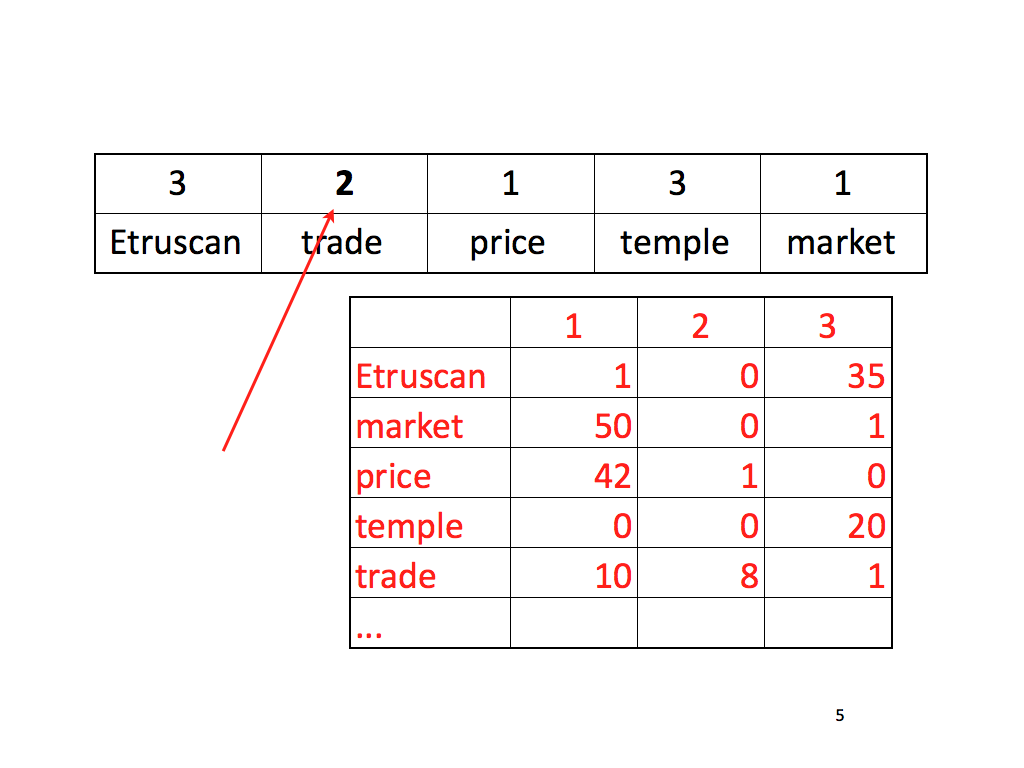
\includegraphics[width=\linewidth]{topic_models/mimno_005}}
    \only<2>{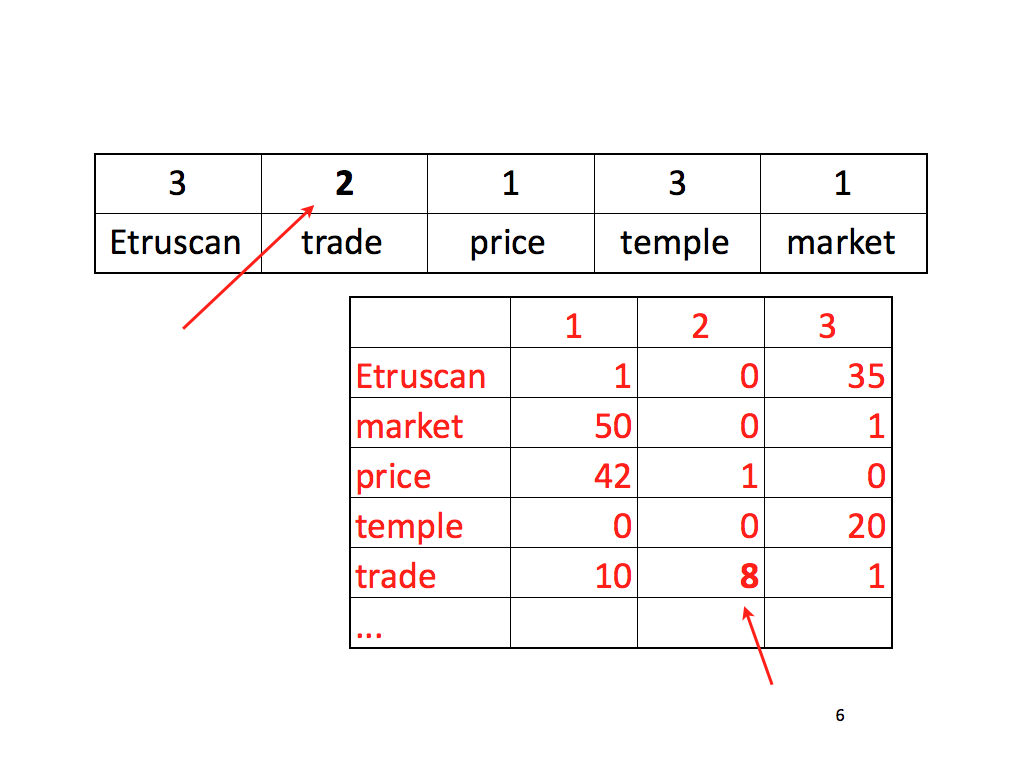
\includegraphics[width=\linewidth]{topic_models/mimno_006}}
\end{frame}

\begin{frame}
  \frametitle{Decrement its count}
    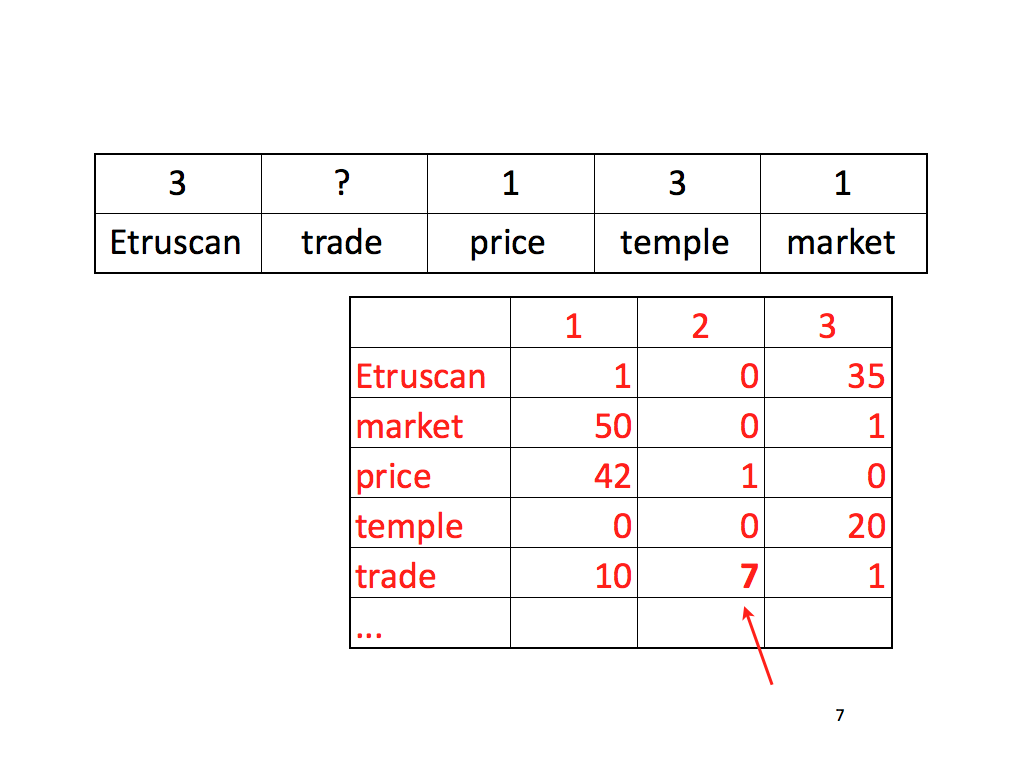
\includegraphics[width=\linewidth]{topic_models/mimno_007}
\end{frame}

\begin{frame}
  \frametitle{What is the conditional distribution for this topic?}
    \includegraphics[width=\linewidth]{topic_models/mimno_008}
\end{frame}


\begin{frame}
  \frametitle{Part 1: How much does this document like each topic?}
    \includegraphics[width=\linewidth]{topic_models/mimno_008}
\end{frame}

\begin{frame}
  \frametitle{Part 1: How much does this document like each topic?}
    \includegraphics[width=\linewidth]{topic_models/mimno_009}

    \pause
    \vspace{-4cm}
    \begin{block}{Sampling Equation}
	\begin{equation*}
          \frac{\alert<3>{n_{d, k}} + \alpha_k}{ \sum_{i}^{K} { \alert<3>{n_{d,i}} + \alpha_i}} \frac{v_{k, w_{d,n}} + \lambda_{w_{d,n}}}{ \sum_{i} { v_{k,i} + \lambda_{i} }}
	\end{equation*}
     \end{block}


\end{frame}


\begin{frame}
  \frametitle{Part 2: How much does each topic like the word?}
    \includegraphics[width=\linewidth]{topic_models/mimno_010}

\pause

\vspace{-3cm}

\begin{block}{Sampling Equation}
	\begin{equation*}
          \frac{n_{d, k} + \alpha_k}{ \sum_{i}^{K} { n_{d,i} + \alpha_i}} \frac{\alert<3>{v_{k, w_{d,n}}} + \lambda_{w_{d,n}}}{ \sum_{i} { \alert<3>{v_{k,i}} + \lambda_{i} }}
	\end{equation*}
\end{block}

\end{frame}


\begin{frame}
  \frametitle{Geometric interpretation}
    \only<1>{\includegraphics[width=\linewidth]{topic_models/mimno_011}}
    \only<2>{\includegraphics[width=\linewidth]{topic_models/mimno_012}}
    \only<3>{\includegraphics[width=\linewidth]{topic_models/mimno_013}}
\end{frame}

\begin{frame}
  \frametitle{Update counts}
    \only<1>{\includegraphics[width=\linewidth]{topic_models/mimno_014}}
    \only<2>{\includegraphics[width=\linewidth]{topic_models/mimno_015}}
    \only<3>{\includegraphics[width=\linewidth]{topic_models/mimno_016}}
\end{frame}


\begin{frame}
  \frametitle{Details: how to sample from a distribution}

\begin{center}
  \includegraphics[width=.8\linewidth]{topic_models/sampling_from_distribution}
\end{center}
\end{frame}

\begin{frame}

\begin{block}{Algorithm}
\begin{enumerate}
\item For each iteration $i$:
\begin{enumerate}
\item For each document $d$ and word $n$ currently assigned to $z_{old}$:
\begin{enumerate}
\item Decrement $n_{d,z_{old}}$ and $v_{z_{old}, w_{d,n}}$
\item Sample $z_{new} = k$ with probability proportional to $\frac{n_{d, k} + \alpha_k}{ \sum_{i}^{K} { n_{d,i} + \alpha_i}} \frac{v_{k, w_{d,n}} + \lambda_{w_{d,n}}}{ \sum_{i} { v_{k,i} + \lambda_{i}}}$
\item Increment $n_{d,z_{new}}$ and $v_{z_{new}, w_{d,n}}$
\end{enumerate}
\end{enumerate}
\end{enumerate}
\end{block}

\end{frame}

\begin{frame}

\frametitle{Implementation}

\begin{block}{Algorithm}
\begin{enumerate}
\item For each iteration $i$:
\begin{enumerate}
\item For each document $d$ and word $n$ currently assigned to $z_{old}$:
\begin{enumerate}
\item Decrement $n_{d,z_{old}}$ and $v_{z_{old}, w_{d,n}}$
\item Sample $z_{new} = k$ with probability proportional to $\frac{n_{d, k} + \alpha_k}{ \sum_{i}^{K} { n_{d,i} + \alpha_i}} \frac{v_{k, w_{d,n}} + \lambda_{w_{d,n}}}{ \sum_{i} { v_{k,i} + \lambda_{i}}}$
\item Increment $n_{d,z_{new}}$ and $v_{z_{new}, w_{d,n}}$
\end{enumerate}
\end{enumerate}
\end{enumerate}
\end{block}

\end{frame}


\begin{frame}
\frametitle{Desiderata}
\begin{itemize}
\item Hyperparameters: Sample them too (slice sampling)
\item Initialization: Random
\item Sampling: Until likelihood converges
\item Lag / burn-in: Difference of opinion on this
\item Number of chains: Should do more than one
\end{itemize}
\end{frame}

\begin{frame}
	\frametitle{Available implementations}

	\begin{itemize}
		\item Mallet (http://mallet.cs.umass.edu)
		\item LDAC (http://www.cs.princeton.edu/~blei/lda-c)
		\item Topicmod (http://code.google.com/p/topicmod)
	\end{itemize}
\end{frame}


\begin{frame}
\frametitle{Previous solutions}

\begin{columns}

\column{.5\linewidth}

\begin{block}{\alert<2>{Gibbs Sampling}}

\begin{itemize}
\item Approximately distributed LDA~\cite{newman2009distributed} \\
\item Use sparse $\mathbf{n}$ and $\mathbf{v}$ \cite{yao2009efficient}
\item Metropolis-Hastings, Alias tables. \cite{yuan2015lightlda}.
\end{itemize}

\end{block}

\column{.5\linewidth}

\begin{block}{Variational Inference}

\begin{itemize}
  \item Parallelize e-step, distribute m-step~\cite{zhai-12}
  \item Online~\cite{hoffman-10}
\end{itemize}

\end{block}

\end{columns}

\begin{block}{Others \dots}
  Spectral~\cite{Nguyen:Hu:Boyd-Graber-2014}, NMF
\end{block}

%Don't tackle the whole problem.
%- Very efficient sparse collapsed samplers (still serial) Light-LDA and Sparse-LDA
%- AD-LDA, ignore that the sampler is serial

\end{frame}

\section{Parallel, efficient, and correct samplers}


\begin{frame}
\frametitle{Partially collapsed sampler with Alias tables}
\framesubtitle{Concurrency \cite{magnusson2017sparse}}


\begin{itemize}
\item Two step sampler, do not integrate out $\beta$:
\begin{enumerate}
    \item Sample $z_{id}$ in parallel over documents as
    \[
    p(z_{id}=k|w_{id},\mathbf{z}_{\lnot i,d},\beta_{\cdot,w_{id}})\propto\beta_{k,w_i}\cdot{(\mathbf{n}^{\lnot i}_{d,k}+\alpha)}\,.
    \]
%    \[
%    p(z_{id}=k|w_{id},\mathbf{z}_{\lnot i})\propto\underbrace{\frac{\mathbf{n}_{k,w_{id}}^{\lnot i}+\lambda}{\sum_v^V \mathbf{n}_{k,v}^{\lnot i}+\lambda}}_{\phi_{k,w_i}}\cdot\underbrace{\frac{\mathbf{v}^{\lnot i}_{d,k}+\alpha}{\sum_k^K \mathbf{v}_{d,k}^{\lnot i}+\alpha}}_{\theta_{d,k}}
%    \]
    \item Sample $\beta_{k}$ in parallel over topics as
\[
\beta_k \sim \text{Dir}(\mathbf{v}_{k,\cdot}+\lambda)\,.
\]
\end{enumerate}
\end{itemize}

\end{frame}

\begin{frame}
\frametitle{Partially collapsed sampler with Alias tables}
\framesubtitle{Efficiency (\cite{magnusson2017sparse} inspired by \cite{li2014reducing})}

\begin{itemize}
\item Sampling is dominated by sampling $\mathbf{z}$
\begin{eqnarray*}
p(z_{id}=k|\cdot) & \propto & \beta_{k,w_{i}}\cdot\left(\mathbf{n}^{\lnot i}_{d,k}+\alpha\right)\\
 & = & \underbrace{\beta_{k,w_{i}}\mathbf{n}^{\lnot i}_{d,k}}_{a}+\underbrace{\beta_{k,w_{i}}\alpha}_{b}
\end{eqnarray*}

\item Need to compute the normalization constant per $z_i$
\begin{eqnarray*}
\sigma_i & = \underbrace{\sum^{K_{d}}\beta_{k,w_{i}}\mathbf{n}^{\lnot i}_{d,k}}_{\sigma_{i,a}} +  \underbrace{\sum^{K}\beta_{k,w_{i}}\alpha}_{\sigma_{i,b}}
\end{eqnarray*}

\end{itemize}

\end{frame}

\begin{frame}
\frametitle{Partially collapsed sampler with Alias tables}
\framesubtitle{Efficiency}


\begin{itemize}

\item Sample a topic indicator $z_i$:
\begin{enumerate}
\item Draw a $u_i \sim U(1,\sigma_i)$
\item \texttt{If} $u_i < \sigma_a$ \\
Sample $k$ from Alias table ($\propto \beta_{k,w_{i}}\alpha$)
\item \texttt{Else} \\ Sample from existing topics  in document ($\propto \beta_{k,w_{i}}\mathbf{n}^{\lnot i}_{d,k}$)
\end{enumerate}

\item Amortized complexity $\sim O(\sum^N_i K_{d(i)})$, where $d(i)$ is the document of topic indicator $i$.

\item Good! \\ $N_d$ does not grow with corpus size (but $K$ does).

\end{itemize}

\end{frame}




\begin{frame}
\frametitle{Polya-Urn approximation}
\framesubtitle{\cite{Terenin2018}}

\begin{itemize}
    \item \emph{Problem}: \\ $\mathbf{\beta}$ is dense and $K \times V$
    \item \emph{Solution}: \\ Approximate a Dirichlet with a Poisson Polya Urn.
%    \item Converge to the same distribution as $N \rightarrow \infty$
    \begin{enumerate}
        \item $\mathbf{\beta}$ becomes sparse (less memory needed)
        \item Sampling $\mathbf{\beta}$ is faster \\ using Poisson draws using Alias tables
        \item Sampling $\mathbf{z}$ is faster \\ Only need to iterate over topics that exist in document and non-zero elements in $\mathbf{\beta}$
    \end{enumerate}
\end{itemize}

\end{frame}


\begin{frame}
\frametitle{Large corpora sampling speed}
\framesubtitle{PUBMED corpus, $K=100$ (left) and $K=1000$ (right)}

\includegraphics[width=0.52\textwidth]{magnusson/pubmed_algo-pubmed-100.png}\includegraphics[width=0.52\textwidth]{magnusson/pubmed_algo-pubmed-1000.png}

% Large scale samplers

\end{frame}

\section{Topic Model Application: Framing}

\begin{frame}
\frametitle{Problem: Detecting Framing and Polarization}

\begin{figure}
    \centering
    \includegraphics[width=0.8\textwidth]{magnusson/jimmie2010.jpg}
    \caption{Jimmie \r{A}kesson at the 2010 election.}
\end{figure}

% Research problems - what happens when the Sweden democrats enter the Swedish parliament

% - Immigration is the most prioritized policy area
% Enter 2010, what is the effect in the parliament? Effect on discourse?

\end{frame}

% How?



\begin{frame}
\frametitle{How do we monitor?}

\begin{figure}
    \centering
    \includegraphics[width=0.6\textwidth]{magnusson/Riksdagsbiblioteket_2.JPG}

    \includegraphics[width=0.6\textwidth]{magnusson/triolith1_1200x410.jpg}
\end{figure}

% Corpus size - 300 000 speeches 100m tokens.

\end{frame}


\begin{frame}{Message Matters}

\begin{itemize}
  \item People make radically different decisions based on how information is
  presented~\cite{tversky-92}
  \item Politicians and marketers do this too
\begin{columns}
\column{.45\linewidth}
\begin{block}{Gain frame}
    Flossing your teeth daily removes particles of food in the mouth, avoiding bacteria, which promotes great breath.
\end{block}
\column{.49\linewidth}
\begin{block}{Loss frame}
    If you do not floss your teeth daily, particles of food remain in the mouth, collecting bacteria, which causes bad breath.
\end{block}

\end{columns}
\pause
  \item Can we discover this automatically in political contexts?
\end{itemize}

\end{frame}

\begin{frame}{Example}

    What are your thoughts on the issue of {\bf immigration}?
    \begin{figure}
    \centering
      \includegraphics[width=\textwidth]{teaparty/figures/framing}
    \end{figure}

\end{frame}

\begin{frame}{How can topic models help?}

\begin{center}
\includegraphics[width=0.7\linewidth]{shlda/ideology_topics} \\
\cite{nguyen-13}
\end{center}

\end{frame}


\begin{frame}
% \frametitle{Example of framing}

\begin{quote}
\footnotesize
``Kom inte och prata med mig om flyktingpolitik och att hj\"{a}lpa flyktingar!
Om man sedan i n\"{a}sta andetag p\r{a}st\r{a}r att den flyktinginvandring som
vi har av solidariska sk\"{a}l ocks\r{a} handlar om att r\"{a}dda v\"{a}lf\"{a}rden l\r{a}ngsiktigt
tycker jag att det \"{a}r ett d\r{a}ligt s\"{a}tt att r\"{a}dda v\"{a}lf\"{a}rden p\r{a}, f\"{o}r
det inneb\"{a}r stora kostnader f\"{o}r Sverige i dag. Det inneb\"{a}r s\r{a} stora
kostnader att det faktiskt begr\"{a}nsar v\r{a}r m\"{o}jlighet att uppr\"{a}tth\r{a}lla
och utveckla v\"{a}lf\"{a}rden.''

\bigskip{}

\footnotesize
``{[}Vi{]} st\r{a}r bakom en reglerad invandring. Det betyder att ett
ja \"{a}r ett ja och ett nej \"{a}r ett nej. Men det inneb\"{a}r ocks\r{a} en human
asylpolitik och att verkst\"{a}llighet av myndigheternas beslut, som polisen
i det h\"{a}r fallet har att ut\"{o}va, ska vara i enlighet med b\r{a}de nationella
och internationella normer.''

\end{quote}

\end{frame}


\begin{frame}
\frametitle{Perspective topic model with word seed}

\begin{itemize}
    \item Perspectives (by party)
    \item Word seeds (for one topic)
    \begin{itemize}
        \item flyktingpolitik (refugee policy),
        \item ``flykting (refugee),
        \item asyl (asylum),
        \item migrationsverket (migration board),
        \item invandringspolitik (immigration policy),
        \item invandrare (immigrant) and
        \item integrationspolitik (integration policy)
    \end{itemize}
\end{itemize}

\end{frame}


% What?
\begin{frame}
\frametitle{Result: Immigration topic}

\begin{figure}
    \centering
    \includegraphics[width=1\textwidth]{magnusson/immigration_topics}
\end{figure}

\end{frame}


\begin{frame}
\frametitle{Result: Agenda}

\begin{figure}
    \centering
    \includegraphics[width=1\textwidth]{magnusson/year_debate_topic_prop_tp.png}
    \caption{Immigration topic in Riksdagen 1994-2017}
\end{figure}

\end{frame}


\begin{frame}
\frametitle{Result: Frames}

% latex table generated in R 3.3.2 by xtable 1.8-2 package
% Thu Aug  3 22:54:27 2017
\begin{table}[ht]
\centering
\begin{tabular}{lll}
  \hline
Party & Top words (translated from Swedish)\\
  \hline
  \footnotesize	(s) &   \footnotesize	applies, must, asylum seeker, Swedish Migration Agency* \\
  \footnotesize	(m) & \footnotesize Swedish Migration Agency*, Kalle Larsson, labour migration \\
  \footnotesize	(c) &  \footnotesize Sweden Democrats, here, society, come, Centre Party \\
  \footnotesize (l) & \footnotesize immigrant*, migration minister, refugee policy*, Liberal Party \\
  \footnotesize (v) & \footnotesize day, government, apply, rights, human, right, asylum* \\
  \footnotesize (kd) & \footnotesize Christian Democrats, Barbro Holmberg, generous \\
  \footnotesize (mp) & \footnotesize back, refugees, immensly, children, Europe, send, UNHCR \\
  \footnotesize (sd) & \footnotesize Sweden, will, immigrant*, politics, shall, immigration, Swedish \\
  \hline
\end{tabular}
\caption{Top perspective words by party.}
\label{tab:perspective_topic_types_eng}
\end{table}

\end{frame}


\begin{frame}{Not all \dots}

\begin{itemize}
  \item Further contributions to efficiency
  \item Supervised models for large label sets
  \item Importance of preprocessing
  \item Software Engineering
\end{itemize}

\end{frame}

\begin{frame}{Questions}

  \begin{itemize}
    \item Why Gibbs sampling?
      \pause
    \item Framing / polarization across languages and nations?
      \pause
    \item Importance of interpretability
      \pause
    \item Should all words be uncollapsed?
      \pause
    \item How important is it to be correct?
      \pause
    \item Relationship between latency and throughput
      \pause
    \item Beyond LDA \dots
  \end{itemize}

\end{frame}

\begin{frame}
\bibliographystyle{apalike}
\tiny
\bibliography{bib/journal-full,bib/jbg,magnusson/references}
\end{frame}

\end{document}
